\documentclass[12pt, a4paper, UTF8]{ctexart}
\usepackage{geometry}
\usepackage{graphicx}
\usepackage{booktabs}
\usepackage{xcolor}
\usepackage{float}
\usepackage[hidelinks]{hyperref}
\usepackage{array}
\usepackage{multirow}
\usepackage{caption}
\usepackage{subcaption}

% 页面设置
\geometry{left=2.5cm, right=2.5cm, top=2.5cm, bottom=2.5cm}

% 标题设置
\ctexset{
    section={
        format=\Large\bfseries\centering,
        beforeskip=2ex plus 1ex minus 0.2ex,
        afterskip=2ex plus 0.2ex
    },
    subsection={
        format=\large\bfseries,
        beforeskip=1.5ex plus 1ex minus 0.2ex,
        afterskip=1.5ex plus 0.2ex
    },
    subsubsection={
        format=\normalsize\bfseries,
        beforeskip=1ex plus 0.5ex minus 0.2ex,
        afterskip=1ex plus 0.2ex
    }
}

% 自定义命令

\title{\heiti\zihao{2}制造系统建模与仿真实验报告}
\author{\kaishu\zihao{4}姓名：\underline{\qquad\qquad} \quad 学号：\underline{\qquad\qquad}}
\date{\kaishu\zihao{4}\today}

\begin{document}

% 封面
\begin{titlepage}
    \centering
    \vspace*{2cm}
    {\heiti\zihao{1}\textbf{制造系统建模与仿真}\\[0.5cm]
    \zihao{1}\textbf{实验报告}}\\[2cm]
    {\kaishu\zihao{3}\textbf{实验三：流水线建模与仿真实验}}\\[3cm]
    {\songti\zihao{4}
    \begin{tabular}{lll}
        姓名：\underline{\qquad\qquad\qquad} &
        学号：\underline{\qquad\qquad\qquad} &
        班级：\underline{\qquad\qquad\qquad} \\[0.8cm]
        姓名：\underline{\qquad\qquad\qquad} &
        学号：\underline{\qquad\qquad\qquad} &
        班级：\underline{\qquad\qquad\qquad} \\[0.8cm]
        姓名：\underline{\qquad\qquad\qquad} &
        学号：\underline{\qquad\qquad\qquad} &
        班级：\underline{\qquad\qquad\qquad} \\
    \end{tabular}\\[1.5cm]
    实验日期：\underline{\qquad\qquad\qquad} \quad
    报告日期：\underline{\qquad\qquad\qquad}
    }
    \vfill
\end{titlepage}

% 第一章：实验目的
\section{实验目的}
\begin{enumerate}
    \item 掌握 Part、Machine、Conveyor、Labor 等实体元素和 Variable 逻辑元素的使用方法；
    \item 掌握可视化输入、输出关系的建立方法；
    \item 掌握 Report 工具栏的使用和数据分析方法，进行系统优化设计；
    \item 掌握机器 Breakdown 和 Setup 模式的设计方法；
    \item 熟悉流水线生产系统的运作模式；
    \item 熟悉约束理论及瓶颈转移现象。
\end{enumerate}

% 第二章：实验原理及模型参数
\section{实验原理及模型参数}
\subsection{模型描述}
本实验在 Witness 中构建一条混水线生产系统。零件（widget）依次经过 weigh（称重）、wash（清洗）、produce（加工）、inspect（检测）四道工序，工序间通过 C1、C2、C3 三条传送带运输（容量 20 件，Index Time 0.5 min）。系统中设置了 2 名工人：worker1 负责 weigh 和 produce，worker2 负责 wash 和 inspect。仿真运行时间为 2400 min。

\subsection{模型参数}
\begin{table}[H]
    \centering
    \caption{模型参数设置}
    \begin{tabular}{cccccl}
        \toprule
        工序 & 机器 & 加工时间 (min) & 故障间隔 (min) & 修复时间 (min) & 特殊说明 \\
        \midrule
        称重 & weigh & 5 & 150 & 6 & — \\
        清洗 & wash & 4 & 150 & 6 & — \\
        加工 & produce & 3 & 50 & 10 & 每 10 件 Setup 8 min \\
        检测 & inspect & 3 & 150 & 6 & — \\
        \bottomrule
    \end{tabular}
\end{table}

% 第三章：实验步骤
\section{实验步骤}
\begin{enumerate}
    \item \textbf{建立模型}：在 Witness 中建立 1 个 Part（widget）、4 个 Machine、3 个 Conveyor、2 个 Labor、1 个 Vinteger（ship\_count），模型布局如图 \ref{fig:layout_before}；
    \item \textbf{运行仿真}：仿真时间设为 2400 min，记录各项统计报表；
    \item \textbf{识别瓶颈并改善}：分析 Machine/Conveyor/Labor Statistics，找出瓶颈工序，将 wash 加工时间从 4 min 缩短为 2 min；
    \item \textbf{对比改善前后结果}，验证瓶颈转移；
    \item \textbf{参数敏感性分析}：在改善后模型基础上，分别改变 C1 移位时间（0.5→0.2 min，组1）、produce Setup Time（8→4 min，组2）、produce Breakdown 间隔（50→100 min，组3），观察各参数对系统性能的影响。
\end{enumerate}

\begin{figure}[H]
    \centering
    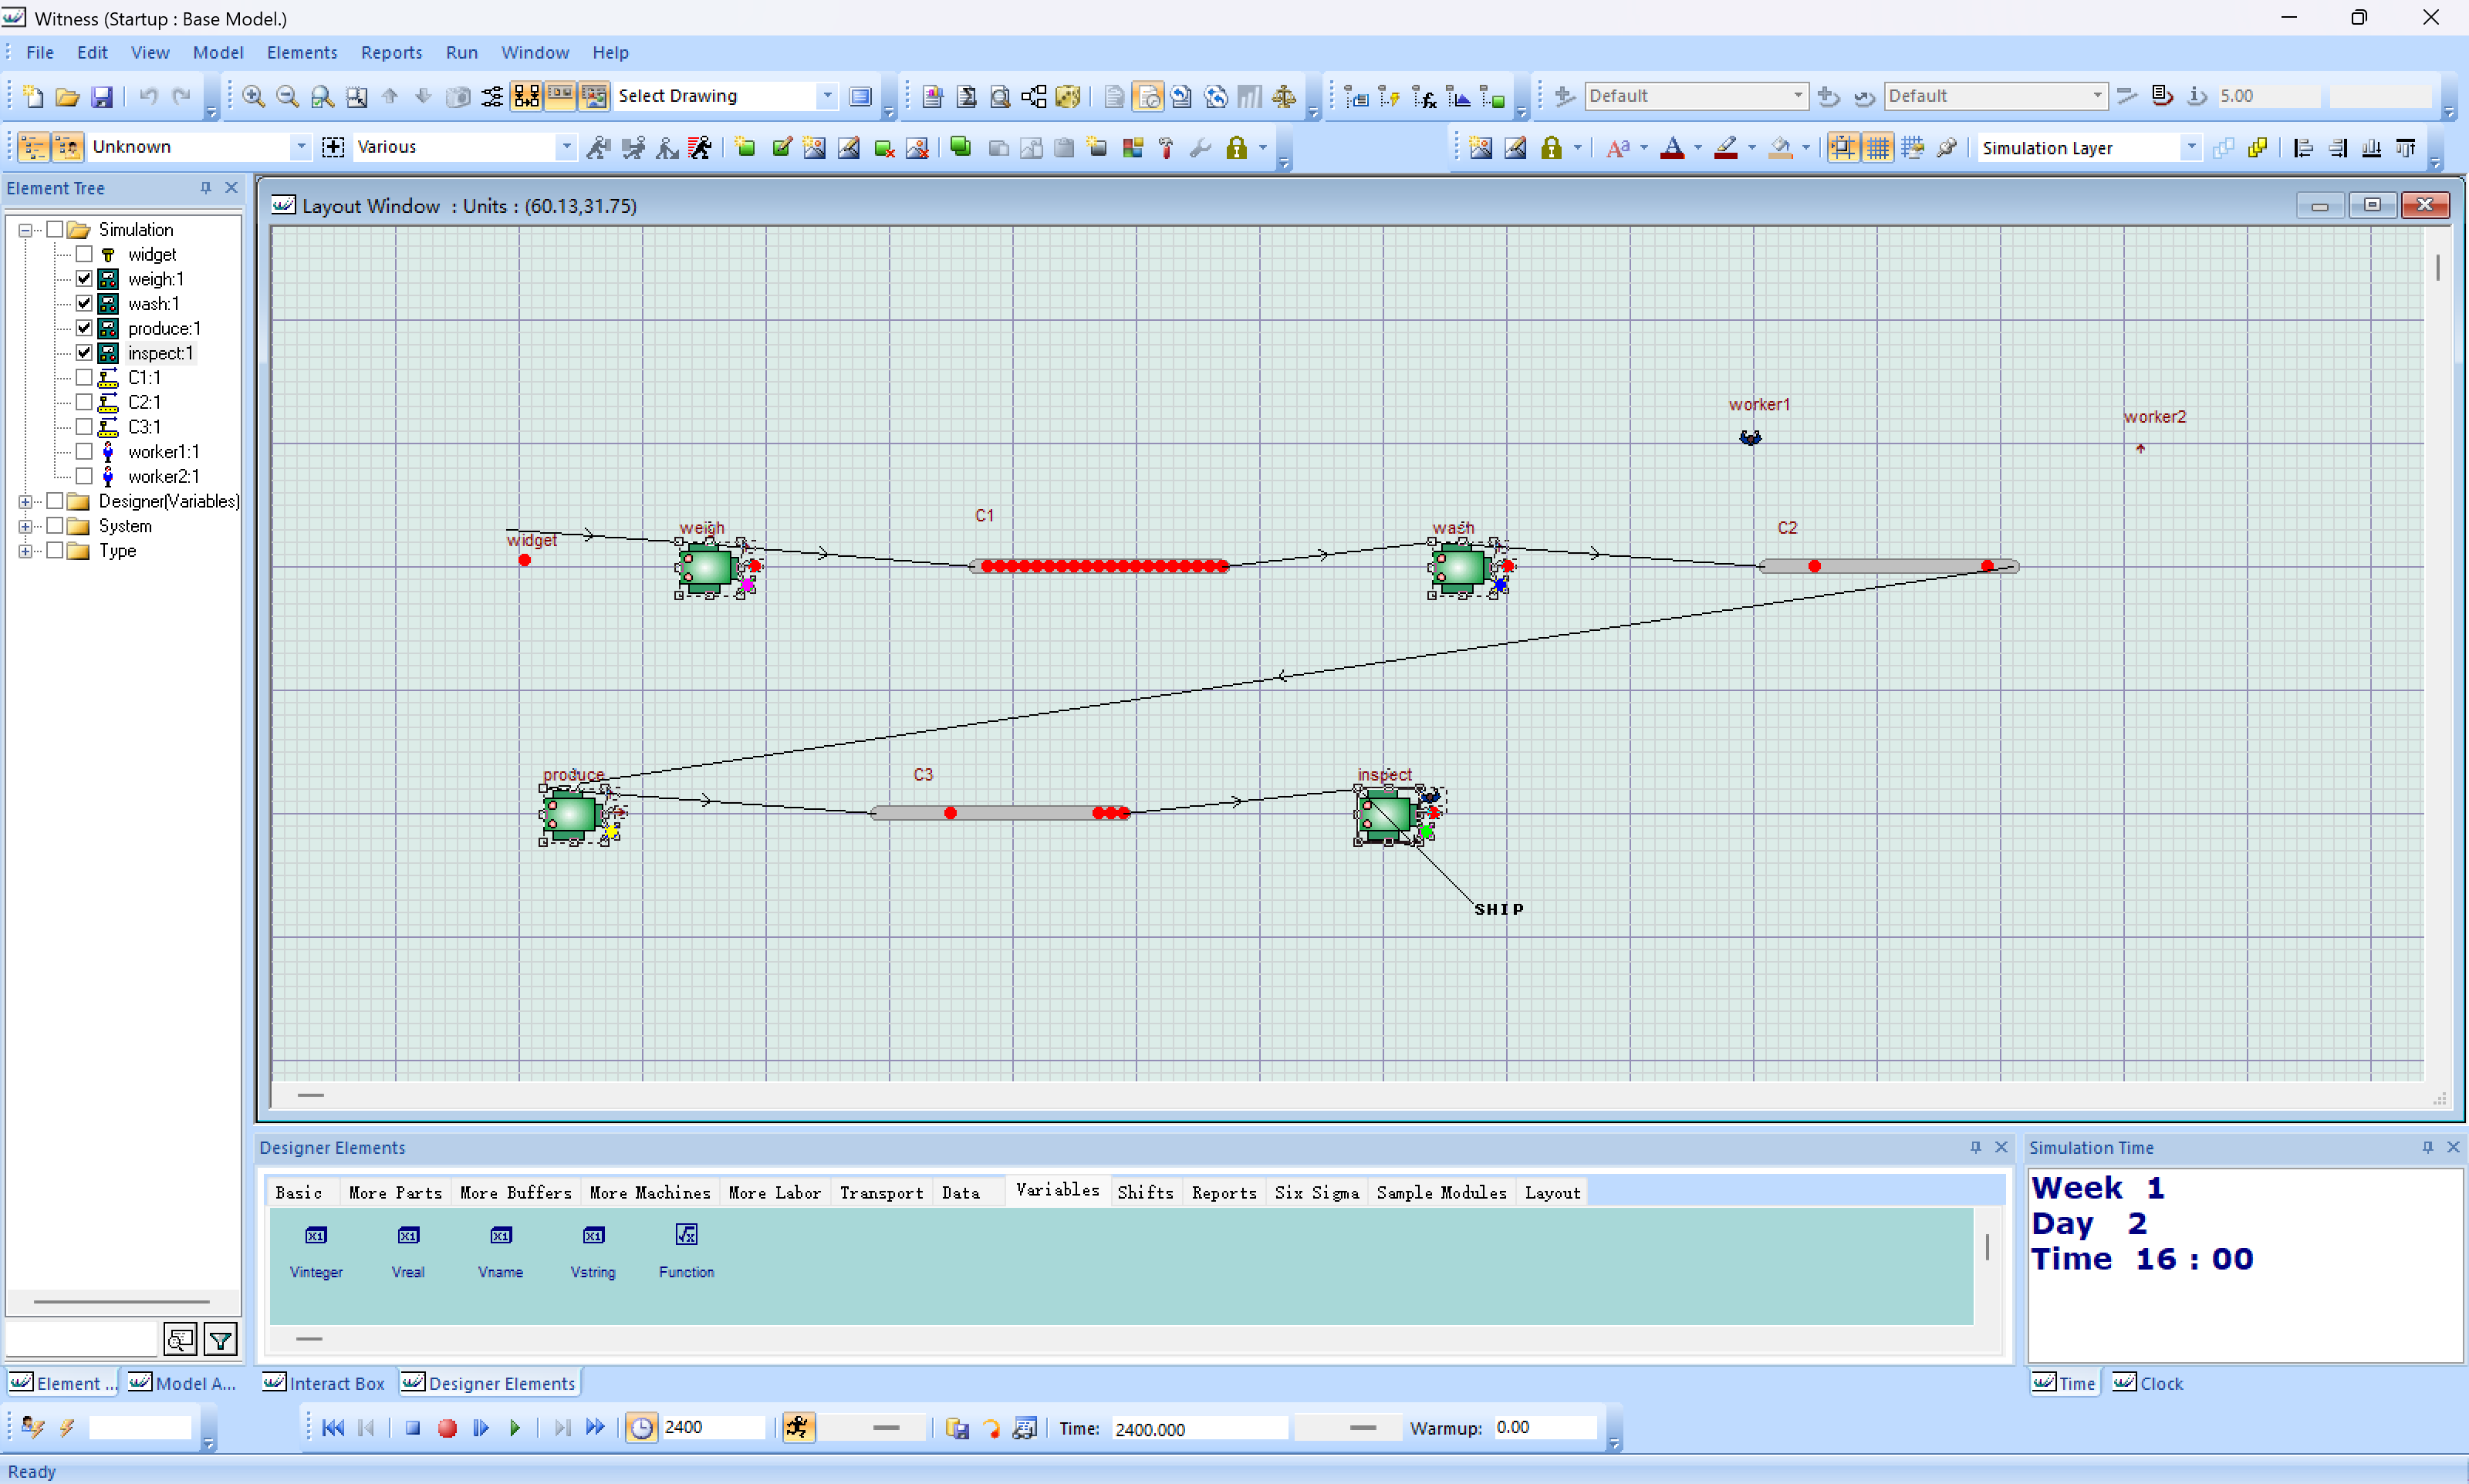
\includegraphics[width=0.75\textwidth]{../实验三_改善前_模型布局.png}
    \caption{实验三模型布局}
    \label{fig:layout_before}
\end{figure}

% 第四章：改善前仿真结果
\section{改善前仿真结果}
按照上述参数运行模型 2400 min，得到各项统计报表，数据汇总于表 \ref{tab:before_all}，原始报表截图见图 \ref{fig:before_screens}。

\smallskip
\noindent\textbf{报表术语说明}：No. Entered（进入数量）、No. Shipped（出货数量）、Avg W.I.P.（平均在制品数）、Avg Time（平均通过时间）；Busy（忙碌率）、Blocked（阻塞率）、Cycle Wait（循环等待率）、Idle（空闲率）、Setup（设置率）、Broken Down（故障率）；Avg Size（传送带平均容量）。下文各表不再重复标注。

\begin{table}[H]
    \centering
    \caption{改善前仿真结果汇总}
    \label{tab:before_all}
    \small
    \begin{tabular}{clcccc}
        \toprule
        \multicolumn{2}{c}{\textbf{Part Statistics}} & \multicolumn{4}{c}{\textbf{Machine Statistics}} \\
        \cmidrule(lr){1-2} \cmidrule(lr){3-6}
        指标 & 数值 & 机器 & Busy & Blocked & Cycle Wait \\
        \midrule
        No. Entered & 366 & weigh & 15.25 & \textbf{84.50} & 0.25 \\
        No. Shipped & 337 & wash & 57.33 & 0.00 & 42.21 \\
        Avg W.I.P. & 28.26 & produce & 42.75 & 0.00 & 0.00 \\
        Avg Time & 185.30 min & inspect & 42.21 & 0.00 & 56.21 \\
        \bottomrule
    \end{tabular}

    \vspace{6pt}
    \small
    \begin{tabular}{clcccc}
        \toprule
        \multicolumn{2}{c}{\textbf{Conveyor Statistics}} & \multicolumn{4}{c}{\textbf{Labor Statistics}} \\
        \cmidrule(lr){1-2} \cmidrule(lr){3-6}
        传送带 & Blocked / Queue & Avg Size & 工人 & Busy & Idle \\
        \midrule
        C1 & \textbf{91.88} / 7.63 & 19.90 & worker1 & 58.00 & 42.00 \\
        C2 & 0.00 / 0.00 & 1.43 & worker2 & \textbf{99.54} & 0.46 \\
        C3 & 0.00 / 98.04 & 3.52 & & & \\
        \bottomrule
    \end{tabular}
\end{table}

从表中可以看到，weigh 的 Blocked 高达 84.50\%，C1 堵塞率更是达到 91.88\%。我们进一步查看 Labor Statistics，发现 worker2 的 Busy 为 99.54\%，几乎一直在工作。这是因为 worker2 同时负责 wash 和 inspect 两道工序，忙不过来，导致 wash 频繁等待工人，零件堆积在 C1 上，weigh 加工完的零件无法送出，所以 weigh 虽然利用率不高却被严重阻塞。因此，wash 环节是系统的瓶颈。

\begin{figure}[H]
    \centering
    \begin{subfigure}{0.48\textwidth}
        \centering
        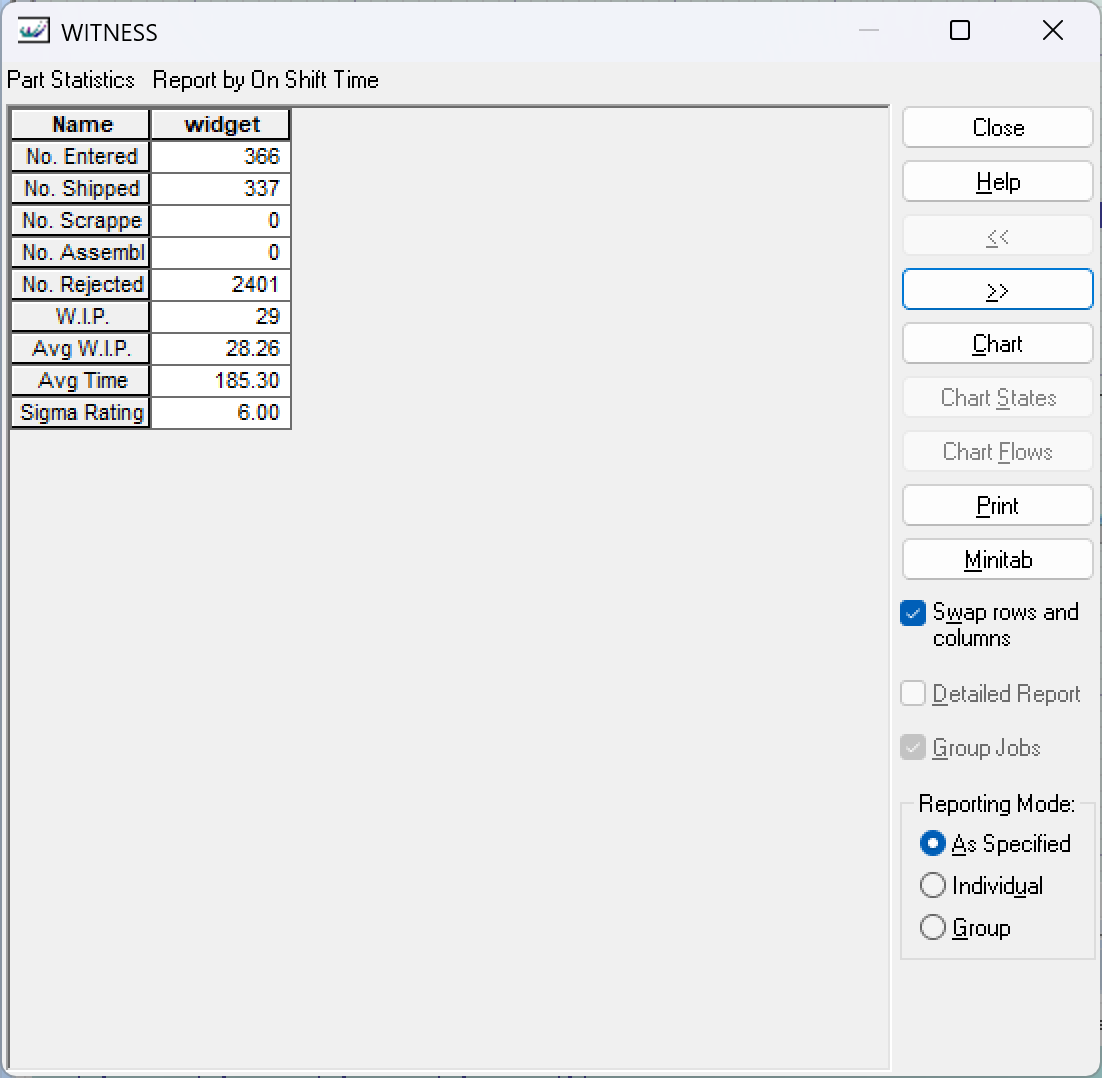
\includegraphics[width=\textwidth]{../实验三_改善前_Part_Statistics.png}
        \caption{Part Statistics}
    \end{subfigure}
    \hfill
    \begin{subfigure}{0.48\textwidth}
        \centering
        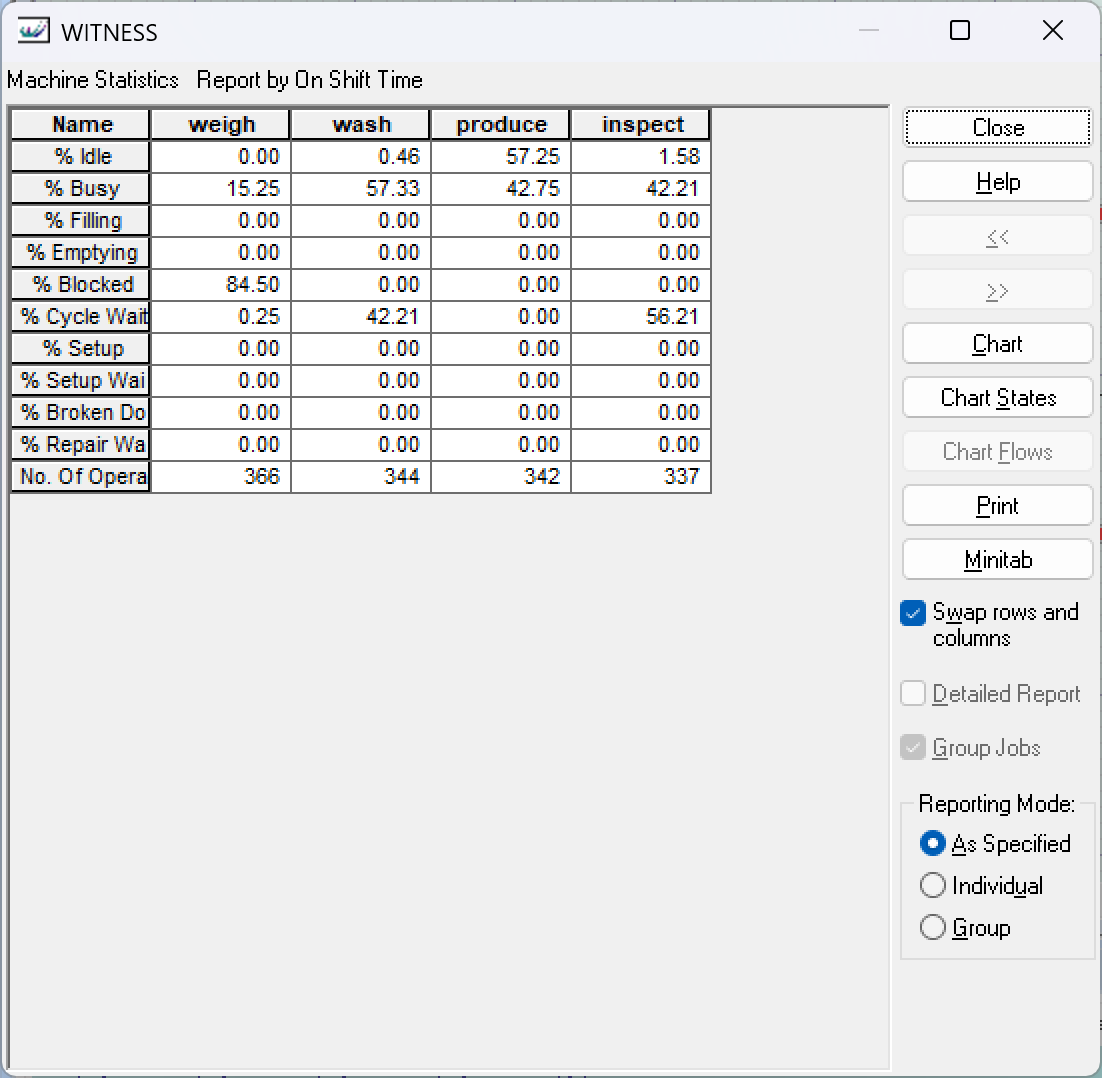
\includegraphics[width=\textwidth]{../实验三_改善前_Machine_Statistics.png}
        \caption{Machine Statistics}
    \end{subfigure}
    \vspace{4pt}
    \begin{subfigure}{0.48\textwidth}
        \centering
        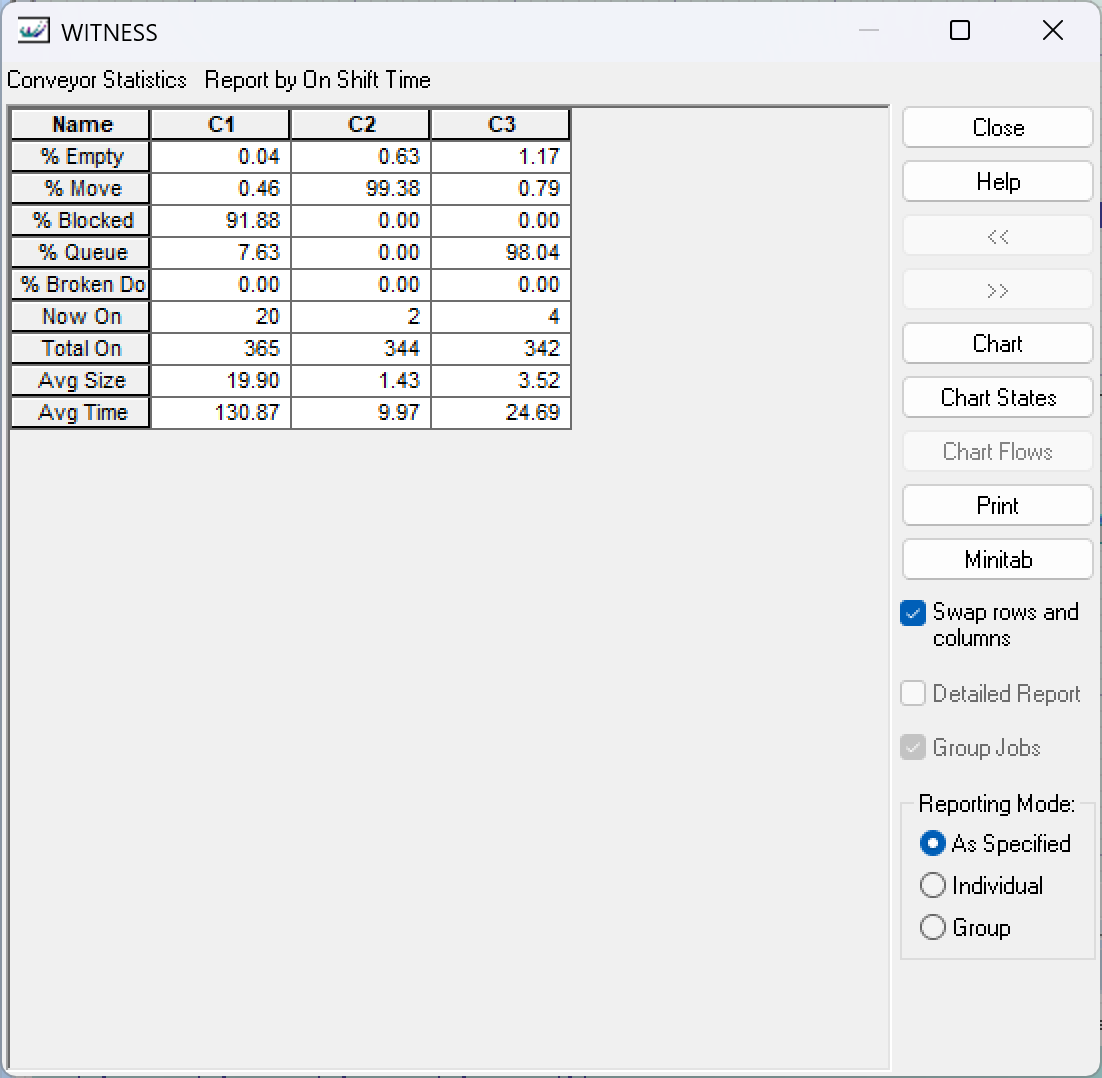
\includegraphics[width=\textwidth]{../实验三_改善前_Conveyor_Statistics.png}
        \caption{Conveyor Statistics}
    \end{subfigure}
    \hfill
    \begin{subfigure}{0.48\textwidth}
        \centering
        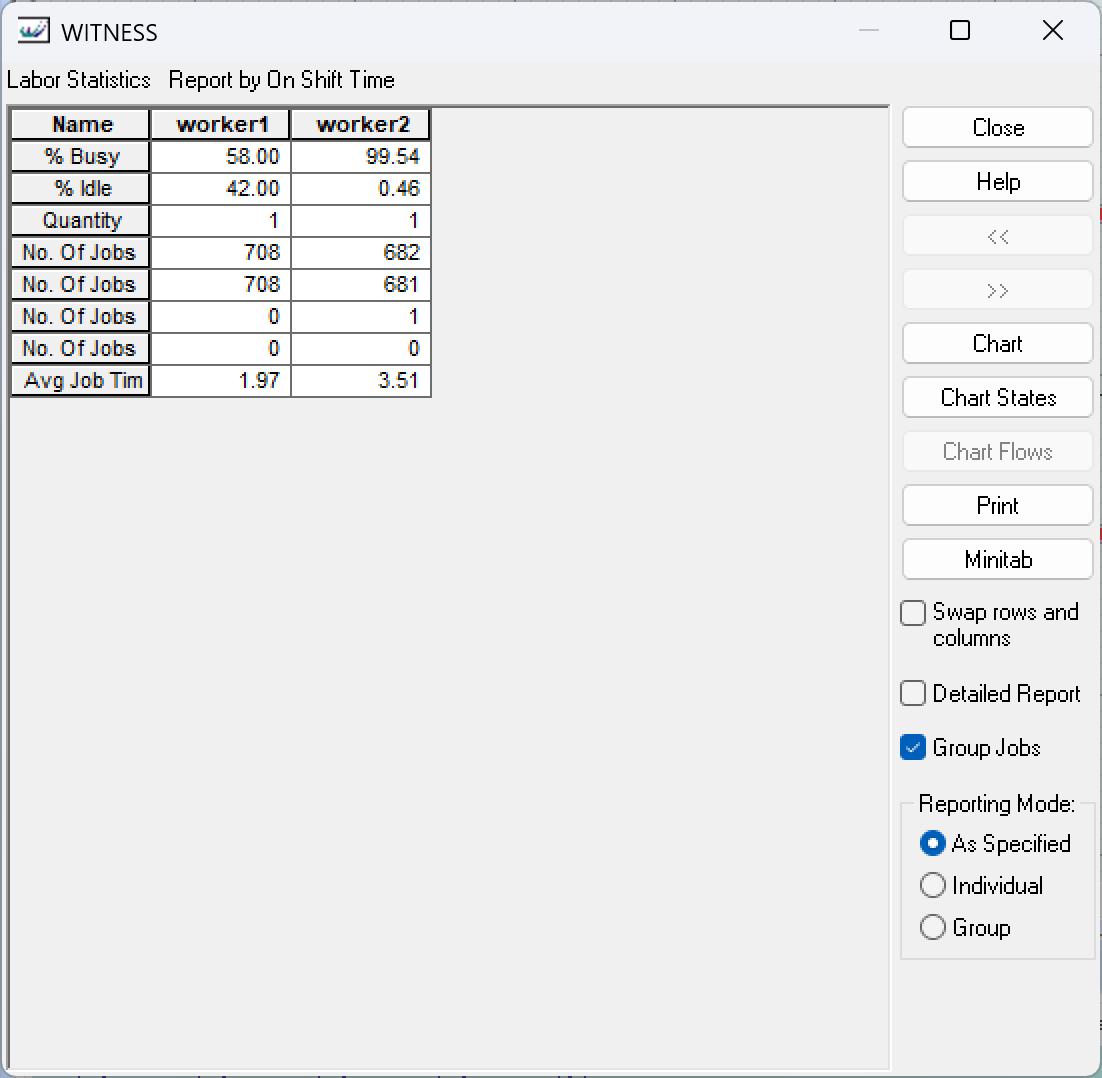
\includegraphics[width=\textwidth]{../实验三_改善前_Labor_Statistics.png}
        \caption{Labor Statistics}
    \end{subfigure}
    \caption{改善前仿真报表截图}
    \label{fig:before_screens}
\end{figure}

% 第五章：瓶颈分析与改善
\section{瓶颈分析与改善}
\subsection{改善措施}
根据上面的分析，wash 是系统瓶颈，因此我们尝试将 wash 的加工时间从 4 min 缩短为 2 min，提高其处理能力，看看能否缓解 C1 堵塞和 weigh 阻塞的问题。

\subsection{改善后仿真结果}
改善后各项统计数据汇总于表 \ref{tab:after_all}，原始报表截图见图 \ref{fig:after_screens}。

\begin{table}[H]
    \centering
    \caption{改善后仿真结果汇总}
    \label{tab:after_all}
    \small
    \begin{tabular}{clcccc}
        \toprule
        \multicolumn{2}{c}{\textbf{Part Statistics}} & \multicolumn{4}{c}{\textbf{Machine Statistics}} \\
        \cmidrule(lr){1-2} \cmidrule(lr){3-6}
        指标 & 数值 & 机器 & Busy & Blocked & Cycle Wait \\
        \midrule
        No. Entered & 507 & weigh & 21.08 & 18.54 & 60.38 \\
        No. Shipped & 473 & wash & 40.42 & 0.00 & 59.13 \\
        Avg W.I.P. & 34.10 & produce & \textbf{60.38} & 0.00 & 1.46 \\
        Avg Time & 161.41 min & inspect & \textbf{59.13} & 0.00 & 39.38 \\
        \bottomrule
    \end{tabular}

    \vspace{6pt}
    \small
    \begin{tabular}{clcccc}
        \toprule
        \multicolumn{2}{c}{\textbf{Conveyor Statistics}} & \multicolumn{4}{c}{\textbf{Labor Statistics}} \\
        \cmidrule(lr){1-2} \cmidrule(lr){3-6}
        传送带 & Blocked / Queue & Avg Size & 工人 & Busy & Idle \\
        \midrule
        C1 & 83.56 / 15.94 & 19.63 & worker1 & 81.46 & 18.54 \\
        C2 & 0.00 / 5.25 & 2.18 & worker2 & \textbf{99.54} & 0.46 \\
        C3 & 0.00 / 97.92 & 8.69 & & & \\
        \bottomrule
    \end{tabular}
\end{table}

\begin{figure}[H]
    \centering
    \begin{subfigure}{0.48\textwidth}
        \centering
        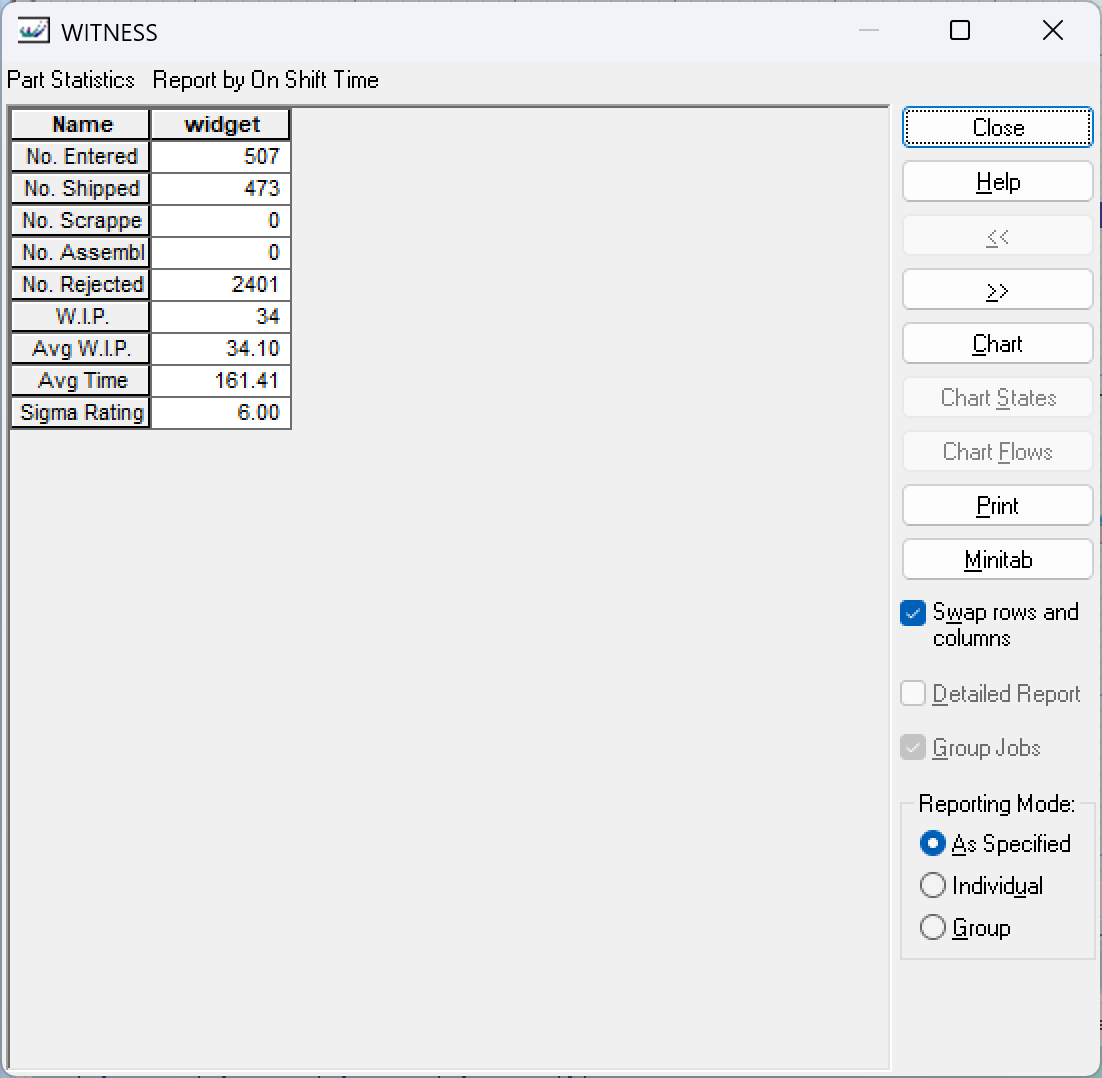
\includegraphics[width=\textwidth]{../实验三_改善后_Part_Statistics.png}
        \caption{Part Statistics}
    \end{subfigure}
    \hfill
    \begin{subfigure}{0.48\textwidth}
        \centering
        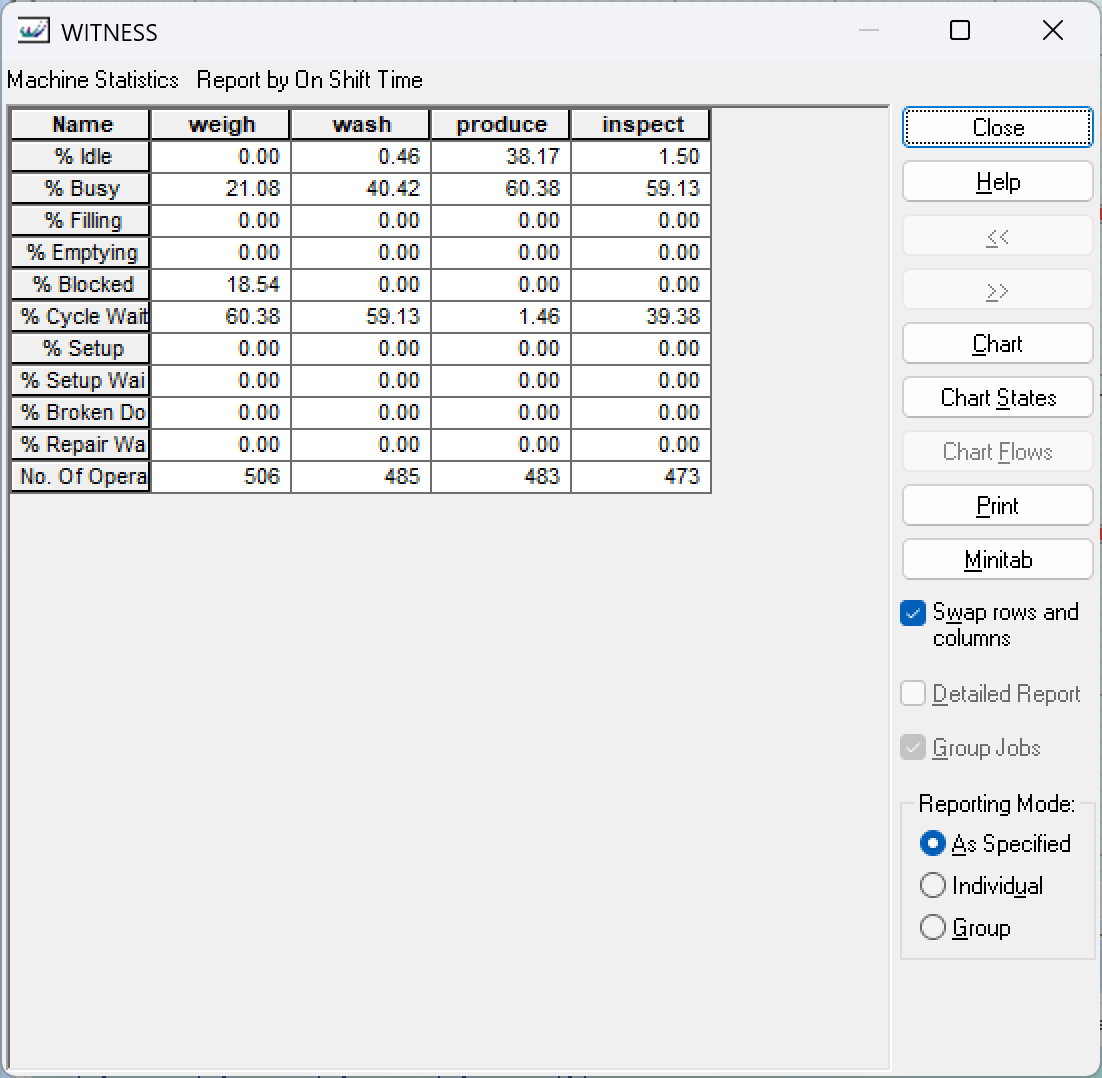
\includegraphics[width=\textwidth]{../实验三_改善后_Machine_Statistics.png}
        \caption{Machine Statistics}
    \end{subfigure}
    \vspace{4pt}
    \begin{subfigure}{0.48\textwidth}
        \centering
        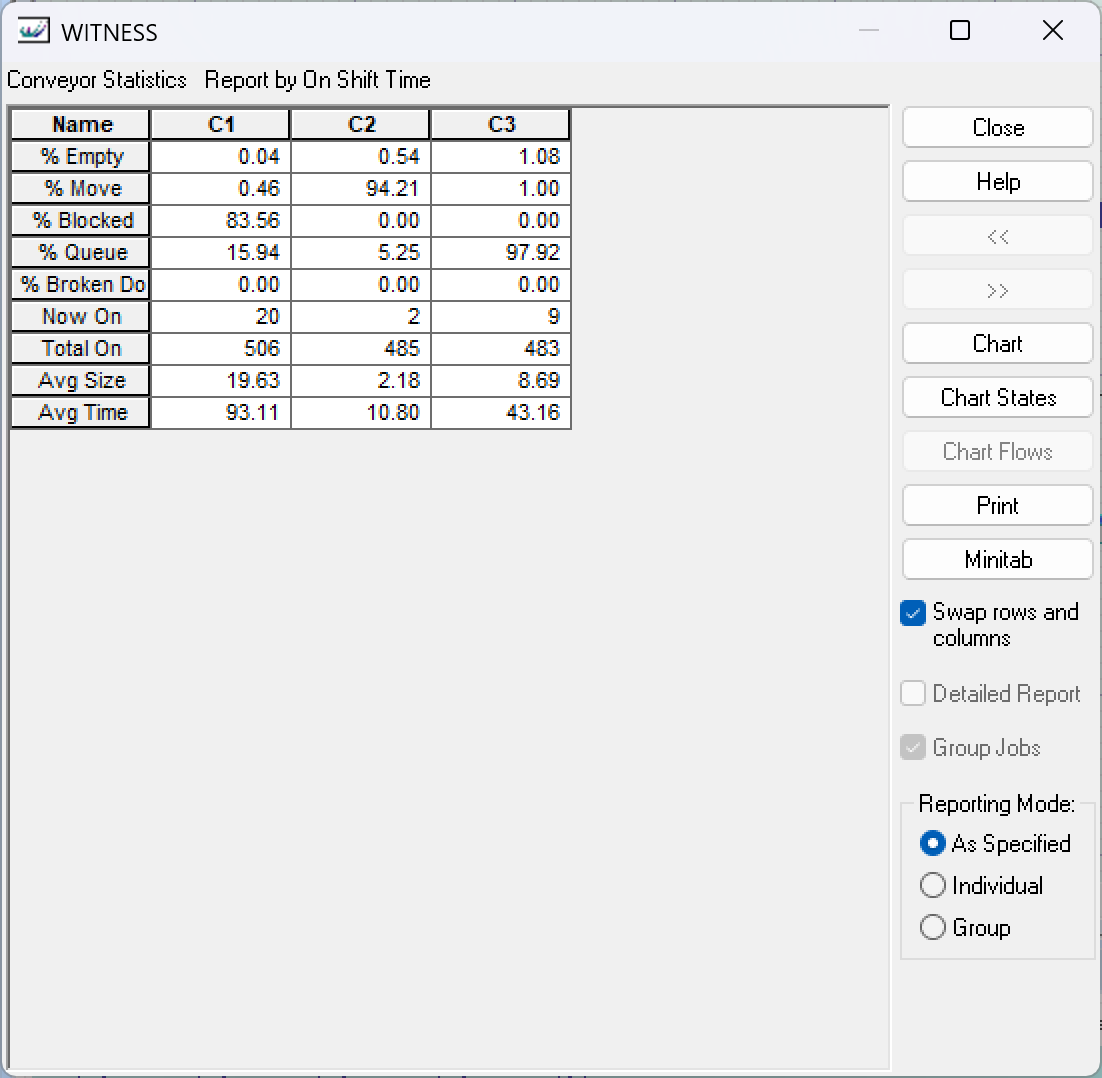
\includegraphics[width=\textwidth]{../实验三_改善后_Conveyor_Statistics.png}
        \caption{Conveyor Statistics}
    \end{subfigure}
    \hfill
    \begin{subfigure}{0.48\textwidth}
        \centering
        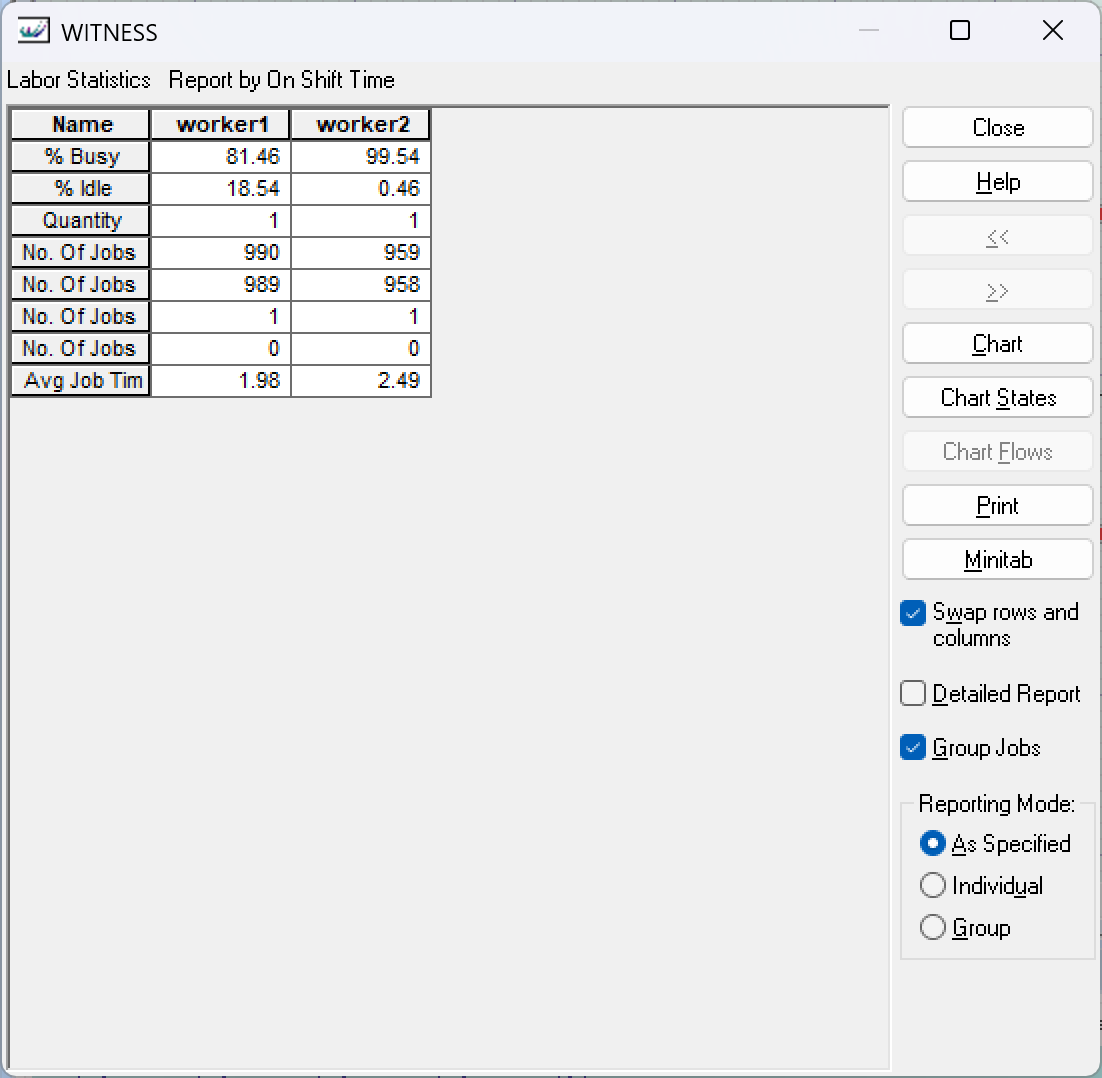
\includegraphics[width=\textwidth]{../实验三_改善后_Labor_Statistics.png}
        \caption{Labor Statistics}
    \end{subfigure}
    \caption{改善后仿真报表截图}
    \label{fig:after_screens}
\end{figure}

\subsection{改善前后对比与瓶颈转移}
我们将改善前后的关键指标整理为表 \ref{tab:comparison} 进行对比。

\begin{table}[H]
    \centering
    \caption{改善前后关键指标对比}
    \label{tab:comparison}
    \small
    \begin{tabular}{lccc}
        \toprule
        \textbf{指标} & \textbf{改善前} & \textbf{改善后} & \textbf{变化} \\
        \midrule
        No. Shipped & 337 & 473 & $+$40.4\% \\
        Avg Time (min) & 185.30 & 161.41 & $-$12.9\% \\
        \midrule
        weigh Busy & 15.25 & 21.08 & $+$5.83 \\
        wash Busy & 57.33 & 40.42 & $-$16.91 \\
        produce Busy & 42.75 & 60.38 & $+$17.63 \\
        inspect Busy & 42.21 & 59.13 & $+$16.92 \\
        \midrule
        weigh Blocked & 84.50 & 18.54 & $-$65.96 \\
        C1 Blocked & 91.88 & 83.56 & $-$8.32 \\
        \midrule
        worker1 Busy & 58.00 & 81.46 & $+$23.46 \\
        worker2 Busy & 99.54 & 99.54 & 不变 \\
        \bottomrule
    \end{tabular}
\end{table}

改善后出货量从 337 件增至 473 件，增长了 40.4\%，平均通过时间也缩短了 12.9\%，效果非常明显。weigh 的 Blocked 从 84.50\% 大幅降至 18.54\%，说明 wash 环节的改善确实缓解了上游的阻塞。

同时我们注意到，produce 的 Busy 从 42.75\% 升至 60.38\%，inspect 从 42.21\% 升至 59.13\%，成为了新的高负荷环节。这说明\textbf{瓶颈已经从 weigh/wash 转移到了 produce/inspect}，正好验证了约束理论的观点：改善一个瓶颈后，系统的瓶颈会转移到其他环节。

另外，worker2 的 Busy 在改善前后都是 99.54\%，一直处于满负荷状态，工人分配不均仍是制约系统性能的根本问题。

% 第六章：参数敏感性分析
\section{参数敏感性分析}
在改善后的模型基础上，我们分别改变三项参数，观察系统性能的变化情况。

\subsection{组1：C1 移位时间 0.5→0.2 min}
将 C1 的 Index Time 从 0.5 min 缩短为 0.2 min，运行结果见表 \ref{tab:group1} 和图 \ref{fig:group1_screens}。

\begin{table}[H]
    \centering
    \caption{组1 仿真结果（C1 Index Time = 0.2 min）}
    \label{tab:group1}
    \small
    \begin{tabular}{clcccc}
        \toprule
        \multicolumn{2}{c}{\textbf{Part Statistics}} & \multicolumn{4}{c}{\textbf{Machine Statistics}} \\
        \cmidrule(lr){1-2} \cmidrule(lr){3-6}
        指标 & 数值 & 机器 & Busy & Blocked & Cycle Wait \\
        \midrule
        No. Entered & 508 & weigh & 21.17 & 18.33 & 60.50 \\
        No. Shipped & 474 & wash & 40.54 & 0.00 & 59.25 \\
        Avg W.I.P. & 33.72 & produce & 60.50 & 0.00 & 1.46 \\
        Avg Time & 159.30 min & inspect & 59.25 & 0.00 & 39.50 \\
        \bottomrule
    \end{tabular}

    \vspace{6pt}
    \small
    \begin{tabular}{clcccc}
        \toprule
        \multicolumn{2}{c}{\textbf{Conveyor Statistics}} & \multicolumn{4}{c}{\textbf{Labor Statistics}} \\
        \cmidrule(lr){1-2} \cmidrule(lr){3-6}
        传送带 & Blocked / Queue & Avg Size & 工人 & Busy & Idle \\
        \midrule
        C1 & 88.19 / 11.56 & 19.22 & worker1 & 81.67 & 18.33 \\
        C2 & 0.00 / 5.25 & 2.19 & worker2 & 99.79 & 0.21 \\
        C3 & 0.00 / 98.17 & 8.71 & & & \\
        \bottomrule
    \end{tabular}
\end{table}

出货量仅从 473 增至 474 件，几乎没有变化，而 C1 的 Blocked 反而从 83.56\% 升到了 88.19\%。这说明\textbf{加快传送带速度并不能解决瓶颈问题}，因为瓶颈在于下游机器的处理能力不足，传送带再快也没用，零件到了下游还是要排队等待。

\begin{figure}[H]
    \centering
    \begin{subfigure}{0.48\textwidth}
        \centering
        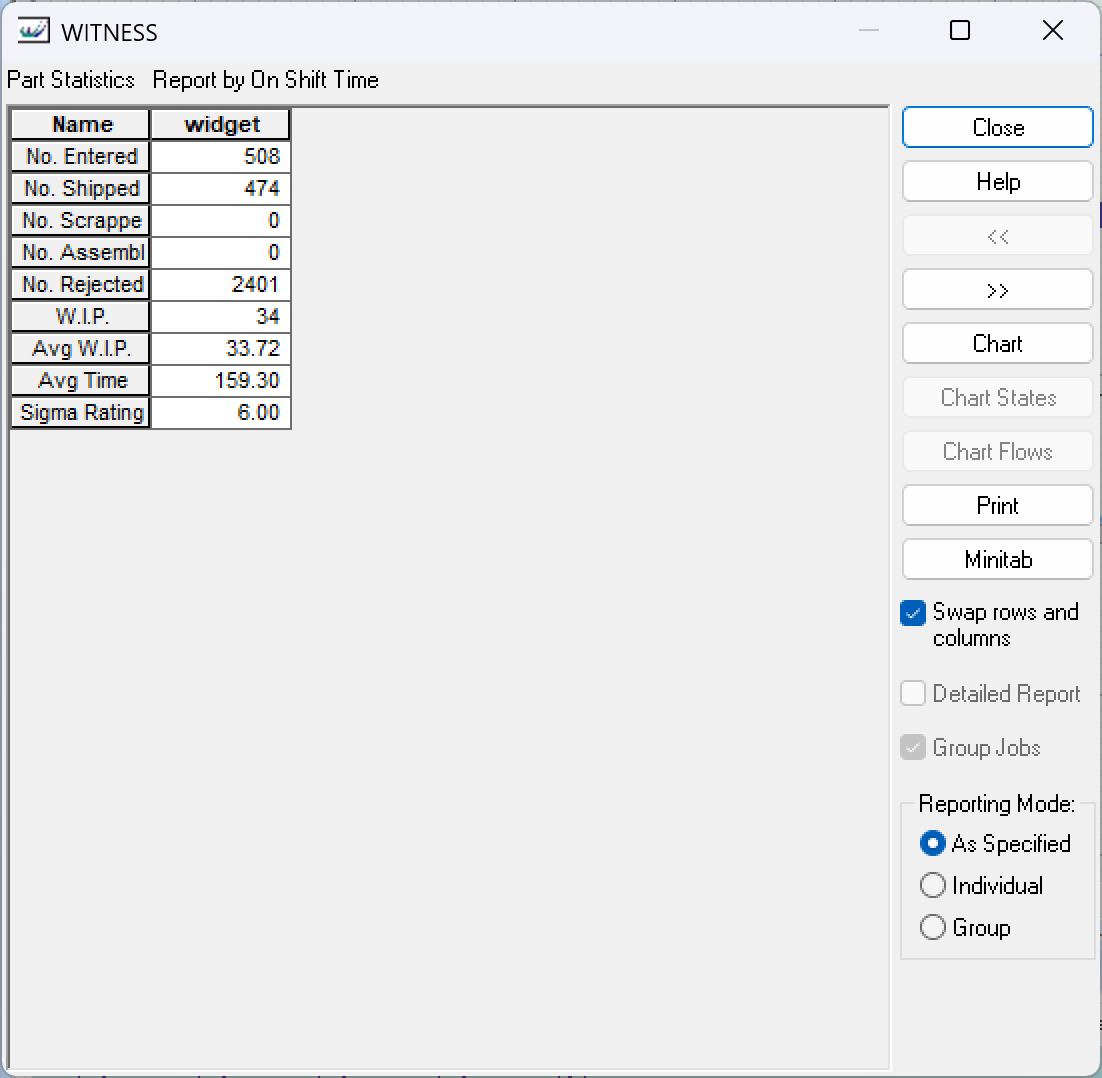
\includegraphics[width=\textwidth]{../组1_Part_Statistics.png}
        \caption{Part Statistics}
    \end{subfigure}
    \hfill
    \begin{subfigure}{0.48\textwidth}
        \centering
        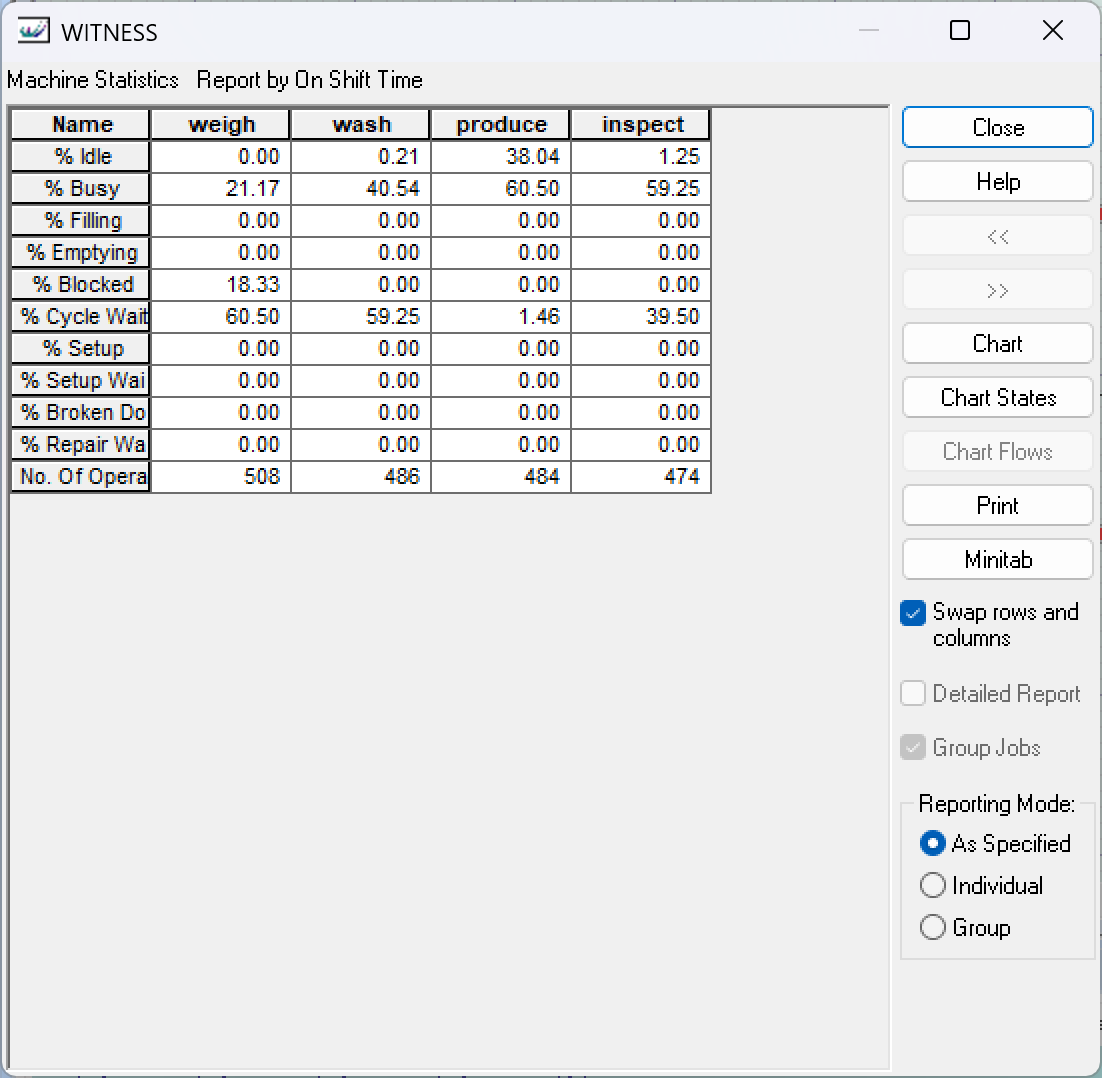
\includegraphics[width=\textwidth]{../组1_Machine_Statistics.png}
        \caption{Machine Statistics}
    \end{subfigure}
    \vspace{4pt}
    \begin{subfigure}{0.48\textwidth}
        \centering
        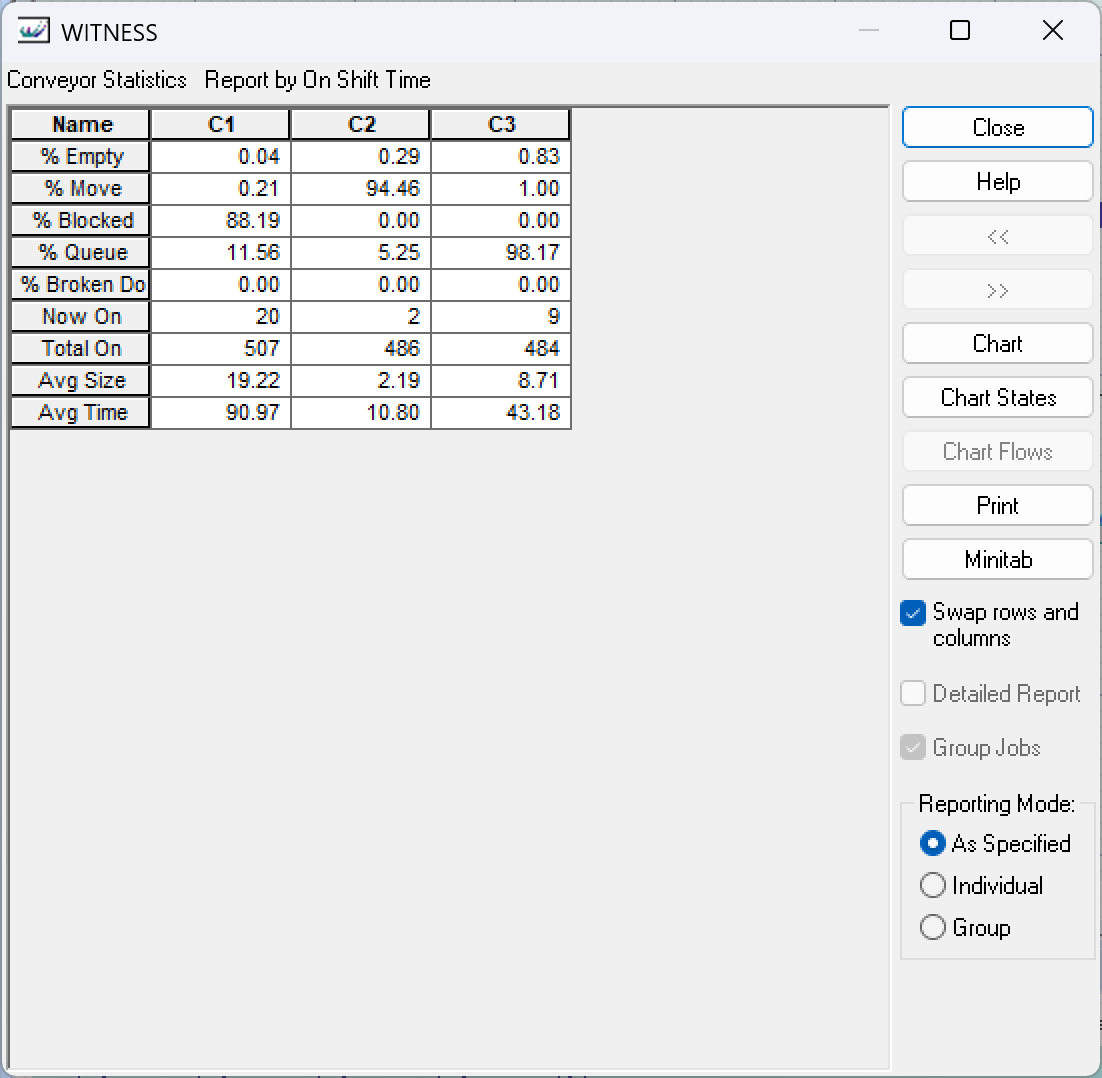
\includegraphics[width=\textwidth]{../组1_Conveyor_Statistics.png}
        \caption{Conveyor Statistics}
    \end{subfigure}
    \hfill
    \begin{subfigure}{0.48\textwidth}
        \centering
        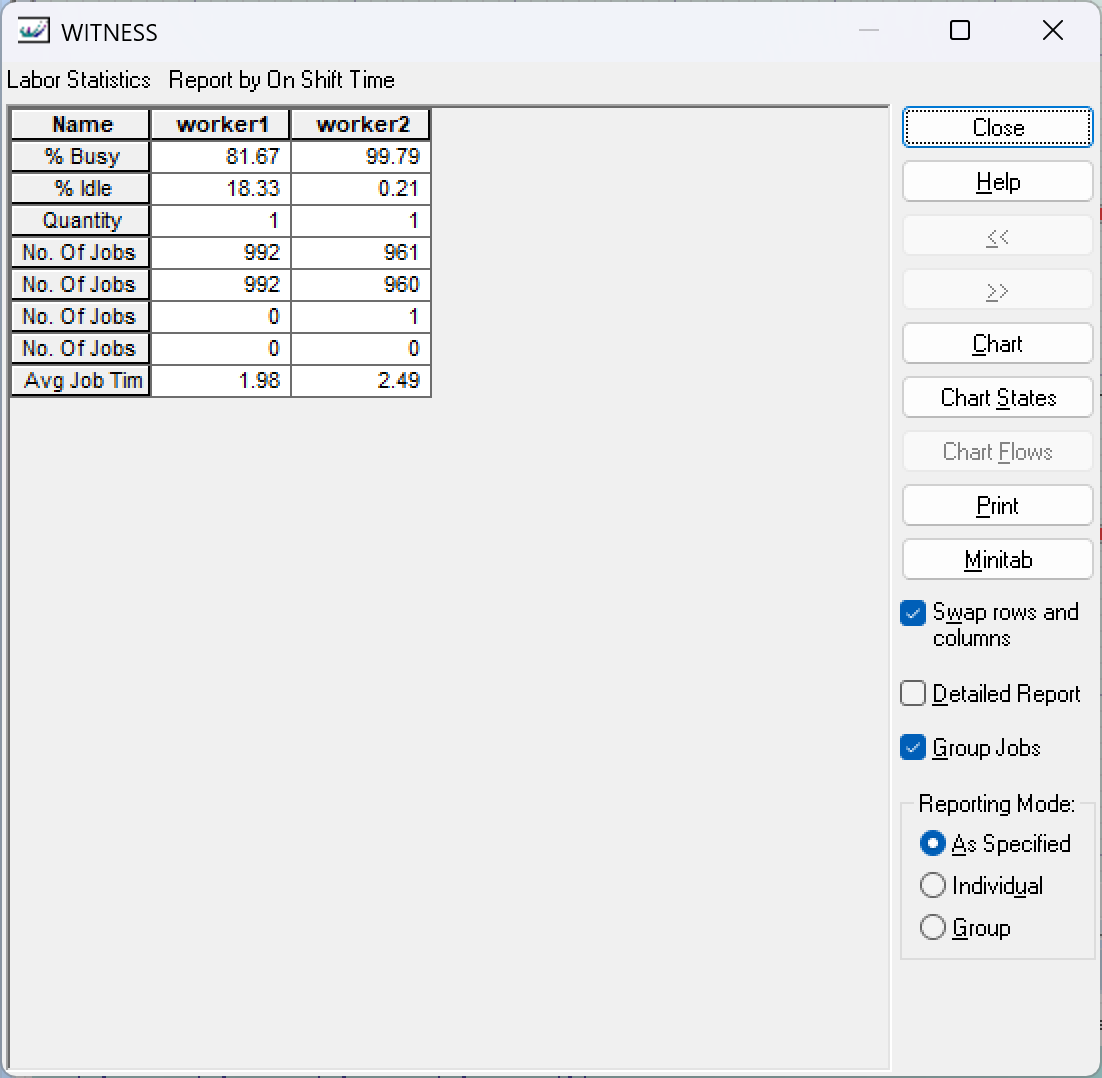
\includegraphics[width=\textwidth]{../组1_Labor_Statistics.png}
        \caption{Labor Statistics}
    \end{subfigure}
    \caption{组1 仿真报表截图（C1 Index Time = 0.2 min）}
    \label{fig:group1_screens}
\end{figure}

\subsection{组2：produce Setup Time 8→4 min}
将 produce 的 Setup Time 从 8 min 缩短为 4 min，结果发现\textbf{各项指标与改善后完全一致}（参见表 \ref{tab:after_all}）。这是因为 produce 的 Setup 为 0.00\%，说明 Setup 并未被触发过，缩短一个没有发生的操作时间自然不会产生任何效果。报表截图见图 \ref{fig:group2_screens}。

\begin{figure}[H]
    \centering
    \begin{subfigure}{0.48\textwidth}
        \centering
        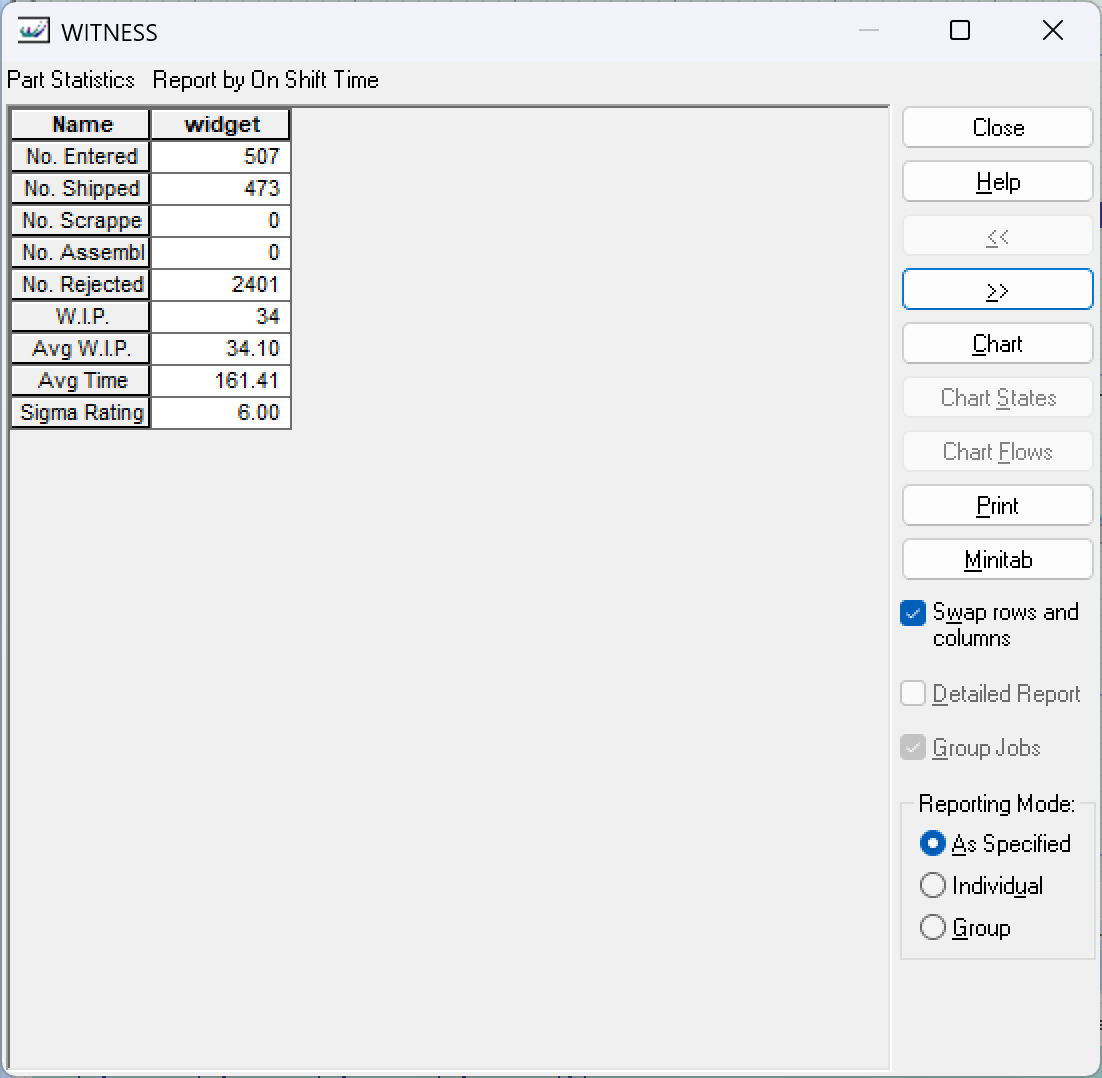
\includegraphics[width=\textwidth]{../组2_Part_Statistics.png}
        \caption{Part Statistics}
    \end{subfigure}
    \hfill
    \begin{subfigure}{0.48\textwidth}
        \centering
        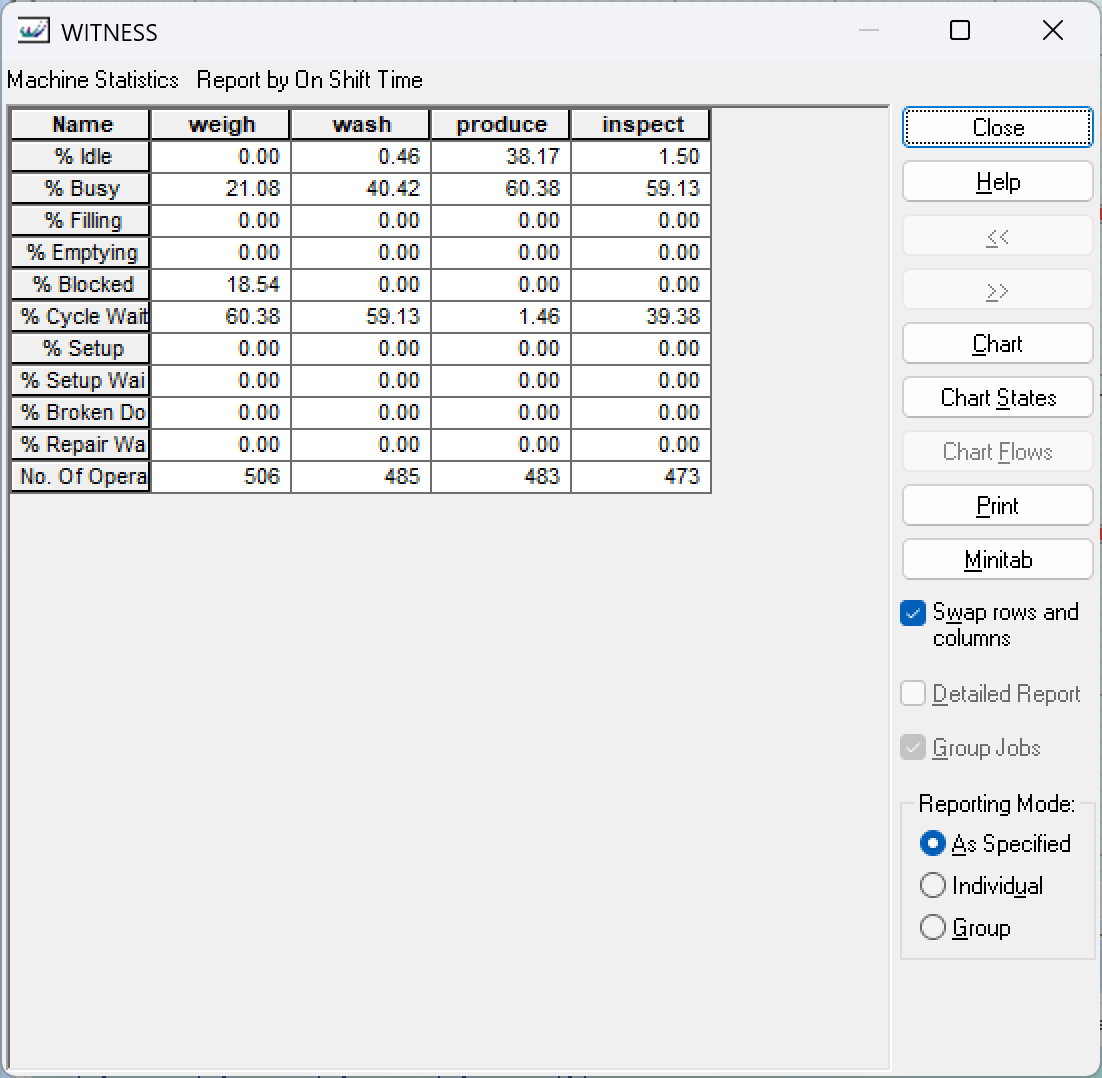
\includegraphics[width=\textwidth]{../组2_Machine_Statistics.png}
        \caption{Machine Statistics}
    \end{subfigure}
    \vspace{4pt}
    \begin{subfigure}{0.48\textwidth}
        \centering
        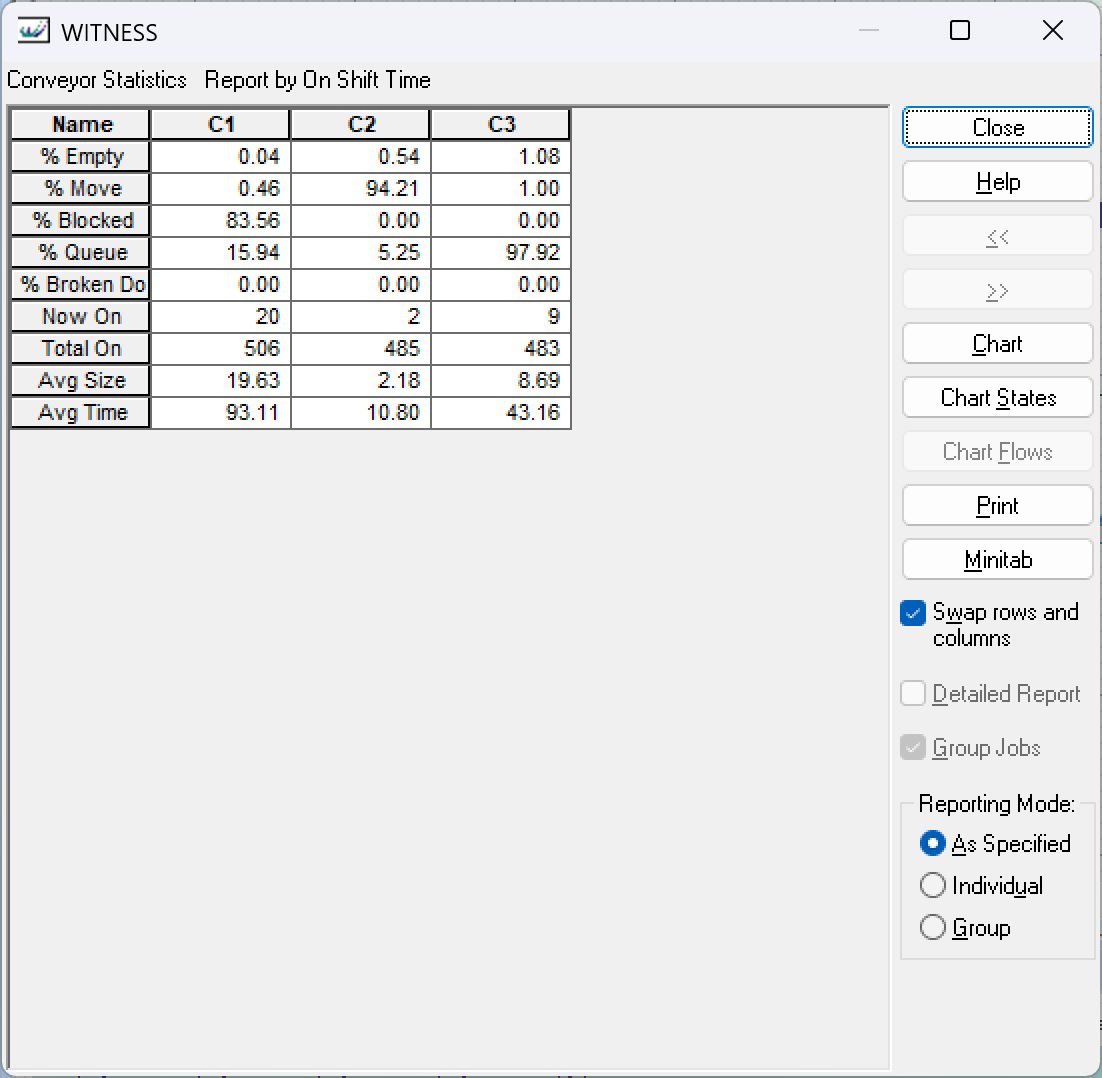
\includegraphics[width=\textwidth]{../组2_Conveyor_Statistics.png}
        \caption{Conveyor Statistics}
    \end{subfigure}
    \hfill
    \begin{subfigure}{0.48\textwidth}
        \centering
        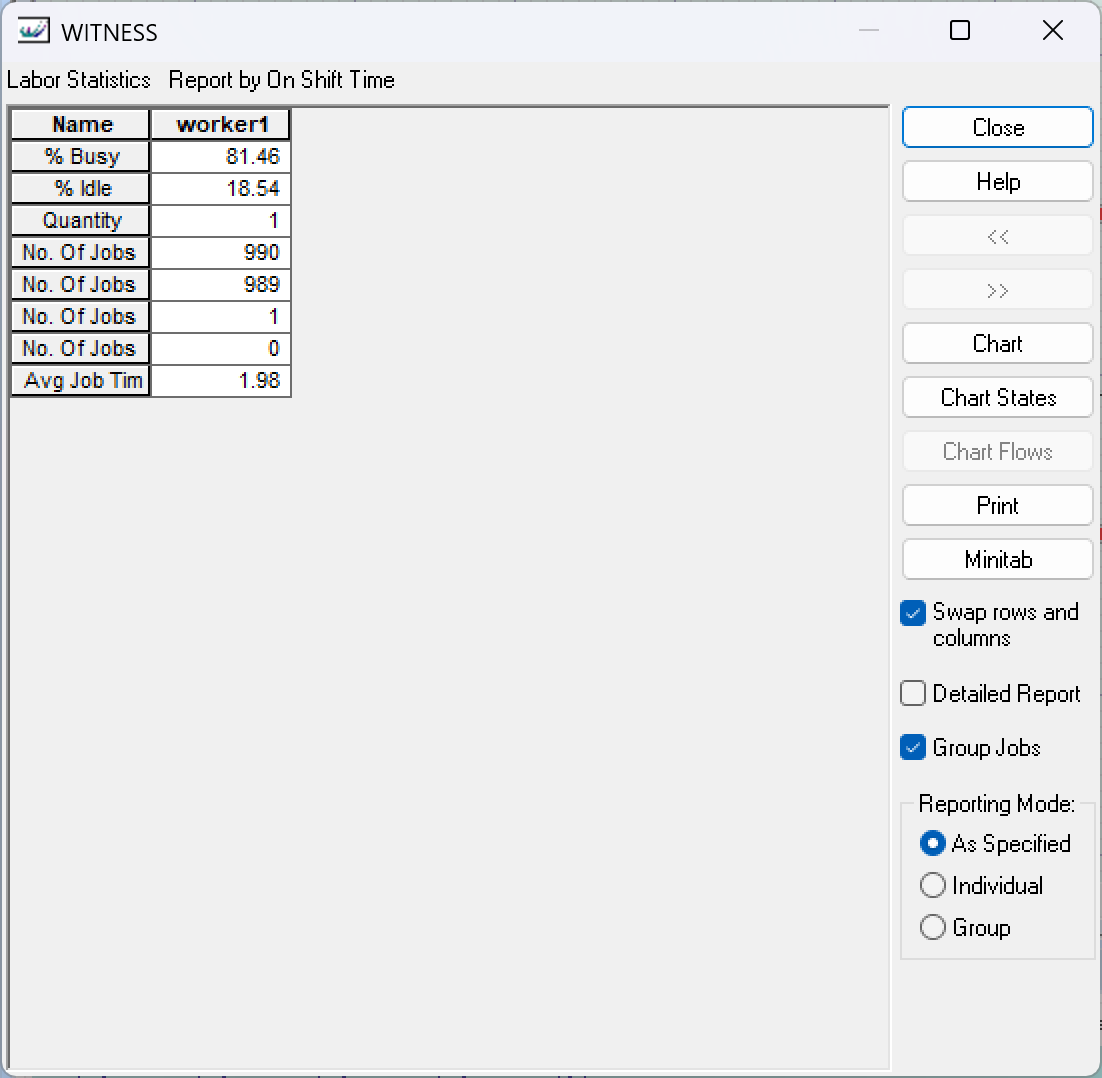
\includegraphics[width=\textwidth]{../组2_Labor_Statistics.png}
        \caption{Labor Statistics}
    \end{subfigure}
    \caption{组2 仿真报表截图（produce Setup Time = 4 min）}
    \label{fig:group2_screens}
\end{figure}

\subsection{组3：produce Breakdown 间隔 50→100 min}
将 produce 的 Breakdown 间隔从 50 min 延长为 100 min，结果\textbf{各项指标同样与改善后完全一致}（参见表 \ref{tab:after_all}）。原因是 produce 的 Broken Down 为 0.00\%，故障本身就没有发生或影响极小，所以延长故障间隔没有任何作用。报表截图见图 \ref{fig:group3_screens}。

\begin{figure}[H]
    \centering
    \begin{subfigure}{0.48\textwidth}
        \centering
        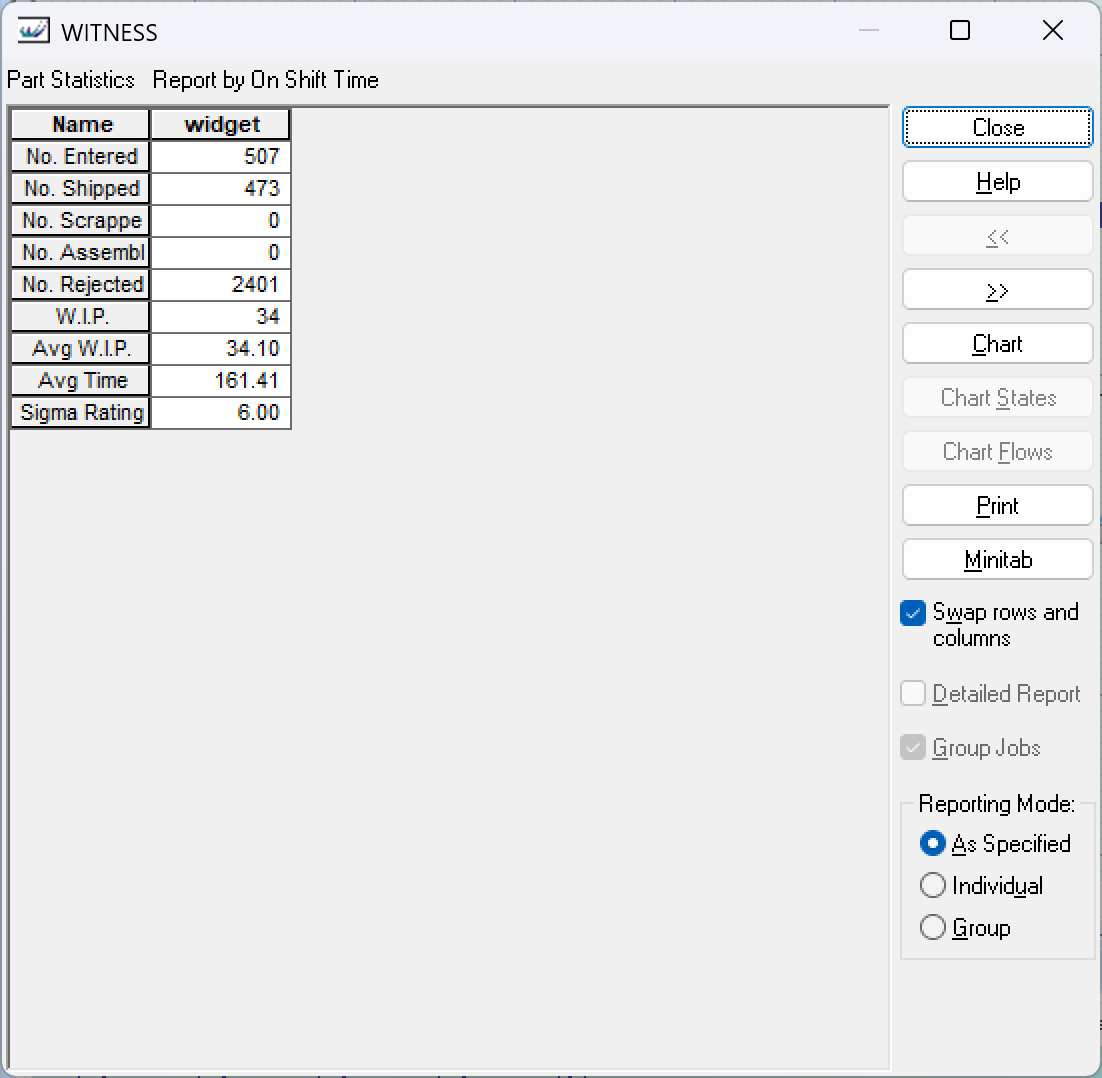
\includegraphics[width=\textwidth]{../组3_Part_Statistics.png}
        \caption{Part Statistics}
    \end{subfigure}
    \hfill
    \begin{subfigure}{0.48\textwidth}
        \centering
        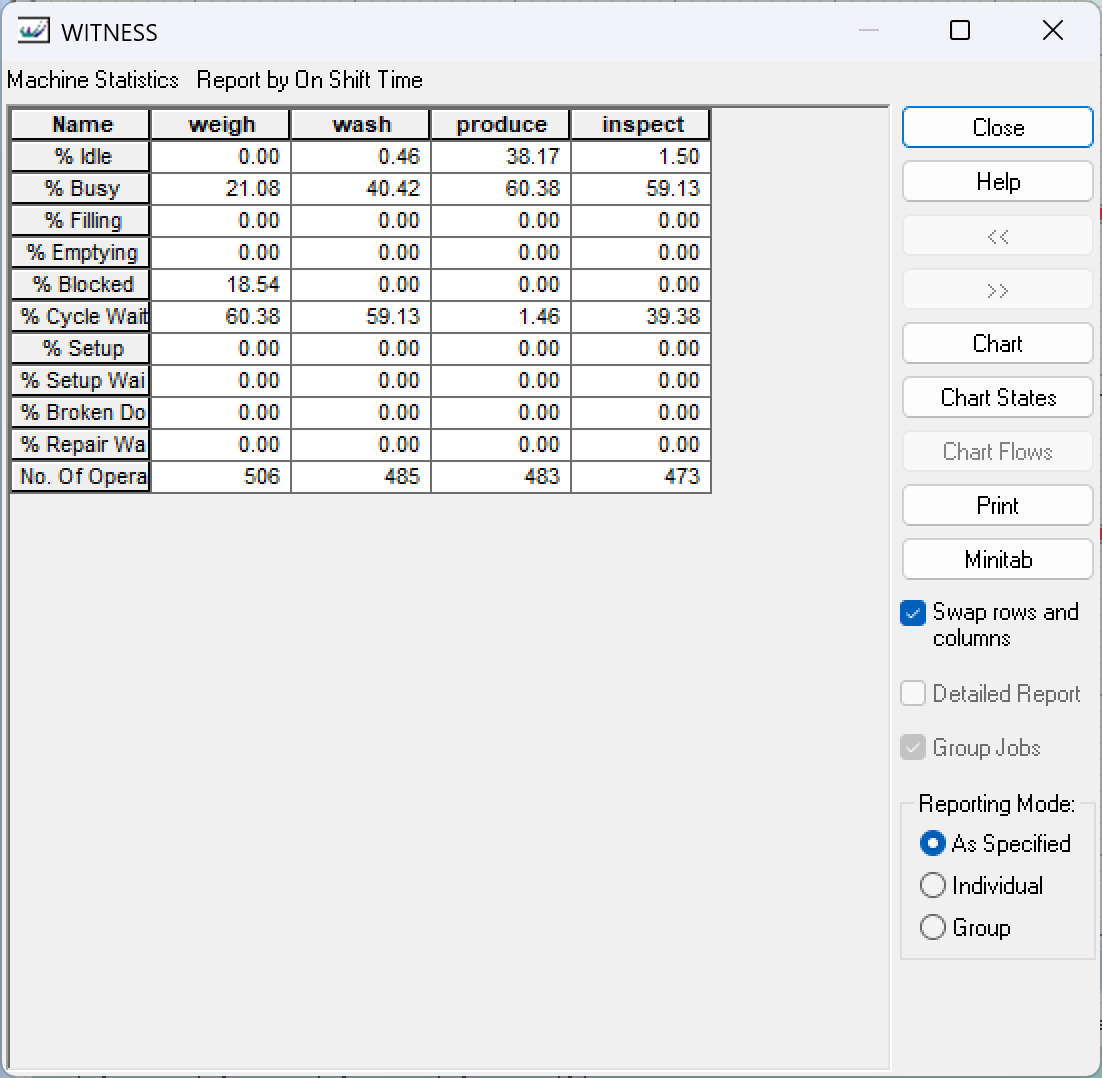
\includegraphics[width=\textwidth]{../组3_Machine_Statistics.png}
        \caption{Machine Statistics}
    \end{subfigure}
    \vspace{4pt}
    \begin{subfigure}{0.48\textwidth}
        \centering
        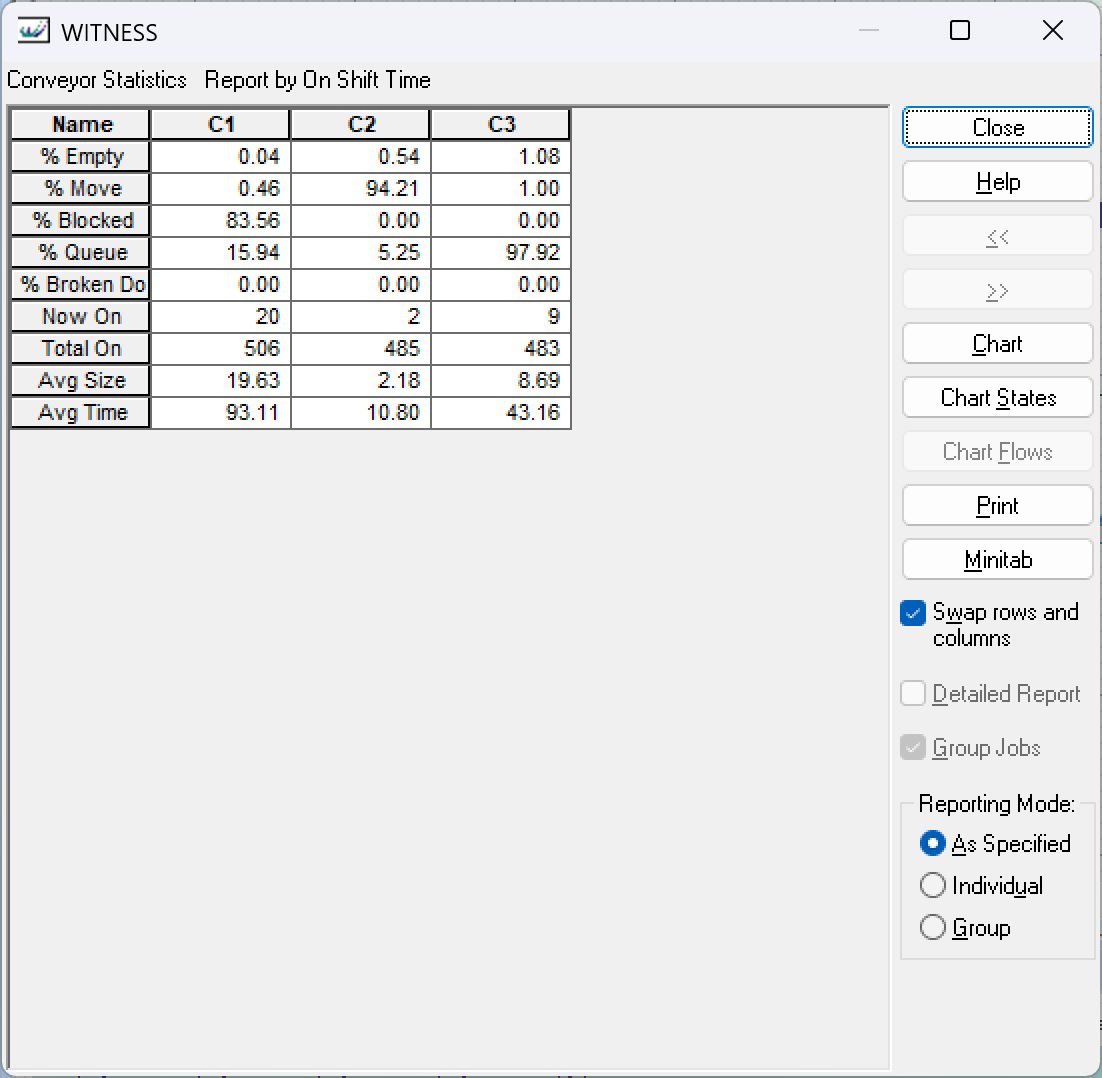
\includegraphics[width=\textwidth]{../组3_Conveyor_Statistics.png}
        \caption{Conveyor Statistics}
    \end{subfigure}
    \hfill
    \begin{subfigure}{0.48\textwidth}
        \centering
        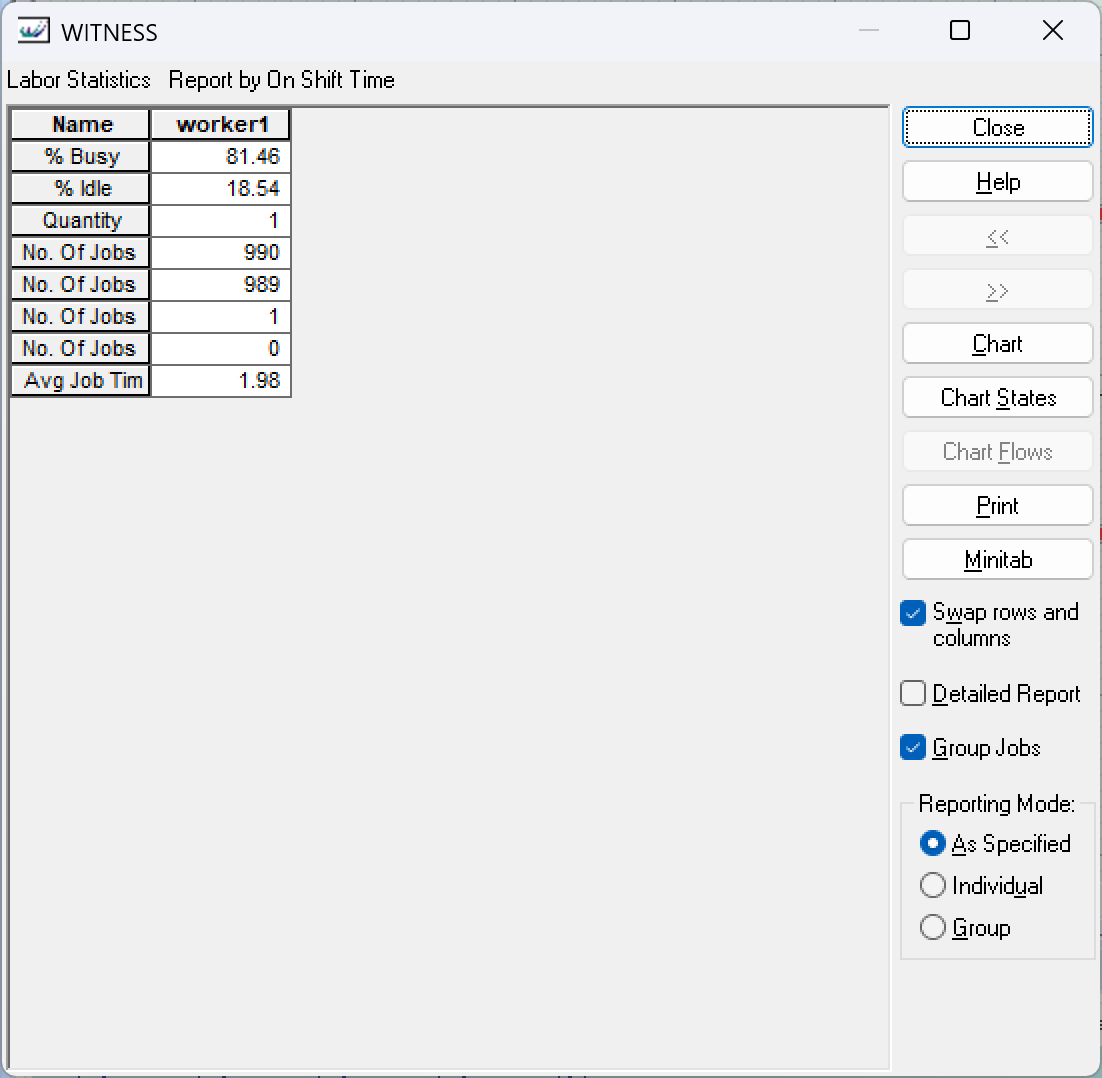
\includegraphics[width=\textwidth]{../组3_Labor_Statistics.png}
        \caption{Labor Statistics}
    \end{subfigure}
    \caption{组3 仿真报表截图（produce Breakdown 间隔 = 100 min）}
    \label{fig:group3_screens}
\end{figure}

\subsection{五组数据综合对比}
我们将改善前、改善后以及三组参数实验的关键指标整理为表 \ref{tab:full_comparison}，方便横向比较。

\begin{table}[H]
    \centering
    \caption{五组实验关键指标综合对比}
    \label{tab:full_comparison}
    \small
    \begin{tabular}{lccccc}
        \toprule
        \textbf{指标} & \textbf{改善前} & \textbf{改善后} & \textbf{组1} & \textbf{组2} & \textbf{组3} \\
        & & wash 2min & C1速度$\uparrow$ & Setup$\downarrow$ & 故障间隔$\uparrow$ \\
        \midrule
        No. Shipped & 337 & 473 & 474 & 473 & 473 \\
        Avg Time (min) & 185.30 & 161.41 & 159.30 & 161.41 & 161.41 \\
        Avg W.I.P. & 28.26 & 34.10 & 33.72 & 34.10 & 34.10 \\
        \midrule
        weigh Busy & 15.25 & 21.08 & 21.17 & 21.08 & 21.08 \\
        wash Busy & 57.33 & 40.42 & 40.54 & 40.42 & 40.42 \\
        produce Busy & 42.75 & 60.38 & 60.50 & 60.38 & 60.38 \\
        inspect Busy & 42.21 & 59.13 & 59.25 & 59.13 & 59.13 \\
        \midrule
        weigh Blocked & 84.50 & 18.54 & 18.33 & 18.54 & 18.54 \\
        C1 Blocked & 91.88 & 83.56 & 88.19 & 83.56 & 83.56 \\
        \midrule
        worker1 Busy & 58.00 & 81.46 & 81.67 & 81.46 & 81.46 \\
        worker2 Busy & 99.54 & 99.54 & 99.79 & 99.54 & 99.54 \\
        \bottomrule
    \end{tabular}
\end{table}

从表 \ref{tab:full_comparison} 可以看出：
\begin{enumerate}
    \item 缩短 wash 加工时间（改善后）效果最显著，出货量增长 40.4\%，瓶颈成功从 wash 转移至 produce/inspect；
    \item 加快 C1 传送带速度（组1）效果很有限，出货仅多 1 件，C1 堵塞率反而更高，说明瓶颈在机器处理能力而不在运输速度；
    \item 缩短 Setup Time（组2）和延长故障间隔（组3）完全没有效果，因为 produce 的 Setup 和 Broken Down 都是 0\%，这两个参数根本没起作用；
    \item 在所有实验中，worker2 的 Busy 始终不低于 99.54\%，工人分配不均是制约系统性能的深层原因。
\end{enumerate}

% 第七章：实验心得体会
\section{实验心得体会}
\begin{enumerate}
    \item 识别瓶颈不能只看机器利用率，要看多个指标综合判断。比如 weigh 的 Busy 只有 15.25\%，看起来很闲，但 Blocked 高达 84.50\%，说明它不是不需要工作，而是被下游堵住了送不出零件。
    \item 找瓶颈要找根本原因，不能只看表面现象。表面上是 weigh 被阻塞，但根因是 worker2 太忙，导致 wash 等待工人，零件堆积在 C1 上。
    \item 瓶颈转移是系统性现象，改善一个瓶颈后会出现新的瓶颈。我们缩短 wash 时间后，produce/inspect 成了新的高负荷环节，这验证了约束理论的核心观点。
    \item 参数敏感性分析帮助我们区分哪些参数对系统有影响、哪些没有。只有针对瓶颈环节的优化才有效，调非瓶颈参数（如组2、组3）是白费功夫。
    \item 工人分配问题贯穿始终，worker2 在所有实验中都接近满负荷，后续可以考虑调整工人分工或增加人手来进一步改善。
\end{enumerate}

\end{document}
